\documentclass[]{book}
\usepackage{lmodern}
\usepackage{amssymb,amsmath}
\usepackage{ifxetex,ifluatex}
\usepackage{fixltx2e} % provides \textsubscript
\ifnum 0\ifxetex 1\fi\ifluatex 1\fi=0 % if pdftex
  \usepackage[T1]{fontenc}
  \usepackage[utf8]{inputenc}
\else % if luatex or xelatex
  \ifxetex
    \usepackage{mathspec}
  \else
    \usepackage{fontspec}
  \fi
  \defaultfontfeatures{Ligatures=TeX,Scale=MatchLowercase}
\fi
% use upquote if available, for straight quotes in verbatim environments
\IfFileExists{upquote.sty}{\usepackage{upquote}}{}
% use microtype if available
\IfFileExists{microtype.sty}{%
\usepackage{microtype}
\UseMicrotypeSet[protrusion]{basicmath} % disable protrusion for tt fonts
}{}
\usepackage[margin=1in]{geometry}
\usepackage{hyperref}
\PassOptionsToPackage{usenames,dvipsnames}{color} % color is loaded by hyperref
\hypersetup{unicode=true,
            pdftitle={A Beginners Guide to R's Galaxy},
            pdfauthor={Michal J. Czyz},
            colorlinks=true,
            linkcolor=blue,
            citecolor=Blue,
            urlcolor=red,
            breaklinks=true}
\urlstyle{same}  % don't use monospace font for urls
\usepackage{natbib}
\bibliographystyle{apalike}
\usepackage{color}
\usepackage{fancyvrb}
\newcommand{\VerbBar}{|}
\newcommand{\VERB}{\Verb[commandchars=\\\{\}]}
\DefineVerbatimEnvironment{Highlighting}{Verbatim}{commandchars=\\\{\}}
% Add ',fontsize=\small' for more characters per line
\usepackage{framed}
\definecolor{shadecolor}{RGB}{255,255,255}
\newenvironment{Shaded}{\begin{snugshade}}{\end{snugshade}}
\newcommand{\KeywordTok}[1]{\textcolor[rgb]{0.12,0.11,0.11}{\textbf{#1}}}
\newcommand{\DataTypeTok}[1]{\textcolor[rgb]{0.00,0.34,0.68}{#1}}
\newcommand{\DecValTok}[1]{\textcolor[rgb]{0.69,0.50,0.00}{#1}}
\newcommand{\BaseNTok}[1]{\textcolor[rgb]{0.69,0.50,0.00}{#1}}
\newcommand{\FloatTok}[1]{\textcolor[rgb]{0.69,0.50,0.00}{#1}}
\newcommand{\ConstantTok}[1]{\textcolor[rgb]{0.67,0.33,0.00}{#1}}
\newcommand{\CharTok}[1]{\textcolor[rgb]{0.57,0.30,0.62}{#1}}
\newcommand{\SpecialCharTok}[1]{\textcolor[rgb]{0.24,0.68,0.91}{#1}}
\newcommand{\StringTok}[1]{\textcolor[rgb]{0.75,0.01,0.01}{#1}}
\newcommand{\VerbatimStringTok}[1]{\textcolor[rgb]{0.75,0.01,0.01}{#1}}
\newcommand{\SpecialStringTok}[1]{\textcolor[rgb]{1.00,0.33,0.00}{#1}}
\newcommand{\ImportTok}[1]{\textcolor[rgb]{1.00,0.33,0.00}{#1}}
\newcommand{\CommentTok}[1]{\textcolor[rgb]{0.54,0.53,0.53}{#1}}
\newcommand{\DocumentationTok}[1]{\textcolor[rgb]{0.38,0.47,0.50}{#1}}
\newcommand{\AnnotationTok}[1]{\textcolor[rgb]{0.79,0.38,0.79}{#1}}
\newcommand{\CommentVarTok}[1]{\textcolor[rgb]{0.00,0.58,1.00}{#1}}
\newcommand{\OtherTok}[1]{\textcolor[rgb]{0.00,0.43,0.16}{#1}}
\newcommand{\FunctionTok}[1]{\textcolor[rgb]{0.39,0.29,0.61}{#1}}
\newcommand{\VariableTok}[1]{\textcolor[rgb]{0.00,0.34,0.68}{#1}}
\newcommand{\ControlFlowTok}[1]{\textcolor[rgb]{0.12,0.11,0.11}{\textbf{#1}}}
\newcommand{\OperatorTok}[1]{\textcolor[rgb]{0.12,0.11,0.11}{#1}}
\newcommand{\BuiltInTok}[1]{\textcolor[rgb]{0.39,0.29,0.61}{\textbf{#1}}}
\newcommand{\ExtensionTok}[1]{\textcolor[rgb]{0.00,0.58,1.00}{\textbf{#1}}}
\newcommand{\PreprocessorTok}[1]{\textcolor[rgb]{0.00,0.43,0.16}{#1}}
\newcommand{\AttributeTok}[1]{\textcolor[rgb]{0.00,0.34,0.68}{#1}}
\newcommand{\RegionMarkerTok}[1]{\textcolor[rgb]{0.00,0.34,0.68}{#1}}
\newcommand{\InformationTok}[1]{\textcolor[rgb]{0.69,0.50,0.00}{#1}}
\newcommand{\WarningTok}[1]{\textcolor[rgb]{0.75,0.01,0.01}{#1}}
\newcommand{\AlertTok}[1]{\textcolor[rgb]{0.75,0.01,0.01}{\textbf{#1}}}
\newcommand{\ErrorTok}[1]{\textcolor[rgb]{0.75,0.01,0.01}{\underline{#1}}}
\newcommand{\NormalTok}[1]{\textcolor[rgb]{0.12,0.11,0.11}{#1}}
\usepackage{longtable,booktabs}
\usepackage{graphicx,grffile}
\makeatletter
\def\maxwidth{\ifdim\Gin@nat@width>\linewidth\linewidth\else\Gin@nat@width\fi}
\def\maxheight{\ifdim\Gin@nat@height>\textheight\textheight\else\Gin@nat@height\fi}
\makeatother
% Scale images if necessary, so that they will not overflow the page
% margins by default, and it is still possible to overwrite the defaults
% using explicit options in \includegraphics[width, height, ...]{}
\setkeys{Gin}{width=\maxwidth,height=\maxheight,keepaspectratio}
\IfFileExists{parskip.sty}{%
\usepackage{parskip}
}{% else
\setlength{\parindent}{0pt}
\setlength{\parskip}{6pt plus 2pt minus 1pt}
}
\setlength{\emergencystretch}{3em}  % prevent overfull lines
\providecommand{\tightlist}{%
  \setlength{\itemsep}{0pt}\setlength{\parskip}{0pt}}
\setcounter{secnumdepth}{5}
% Redefines (sub)paragraphs to behave more like sections
\ifx\paragraph\undefined\else
\let\oldparagraph\paragraph
\renewcommand{\paragraph}[1]{\oldparagraph{#1}\mbox{}}
\fi
\ifx\subparagraph\undefined\else
\let\oldsubparagraph\subparagraph
\renewcommand{\subparagraph}[1]{\oldsubparagraph{#1}\mbox{}}
\fi

%%% Use protect on footnotes to avoid problems with footnotes in titles
\let\rmarkdownfootnote\footnote%
\def\footnote{\protect\rmarkdownfootnote}

%%% Change title format to be more compact
\usepackage{titling}

% Create subtitle command for use in maketitle
\newcommand{\subtitle}[1]{
  \posttitle{
    \begin{center}\large#1\end{center}
    }
}

\setlength{\droptitle}{-2em}
  \title{A Beginners Guide to R's Galaxy}
  \pretitle{\vspace{\droptitle}\centering\huge}
  \posttitle{\par}
  \author{Michal J. Czyz}
  \preauthor{\centering\large\emph}
  \postauthor{\par}
  \predate{\centering\large\emph}
  \postdate{\par}
  \date{2018-02-07}

\usepackage{booktabs}
\usepackage{longtable}

\usepackage{amsthm}
\newtheorem{theorem}{Theorem}[chapter]
\newtheorem{lemma}{Lemma}[chapter]
\theoremstyle{definition}
\newtheorem{definition}{Definition}[chapter]
\newtheorem{corollary}{Corollary}[chapter]
\newtheorem{proposition}{Proposition}[chapter]
\theoremstyle{definition}
\newtheorem{example}{Example}[chapter]
\theoremstyle{definition}
\newtheorem{exercise}{Exercise}[chapter]
\theoremstyle{remark}
\newtheorem*{remark}{Remark}
\newtheorem*{solution}{Solution}
\begin{document}
\maketitle

{
\hypersetup{linkcolor=black}
\setcounter{tocdepth}{1}
\tableofcontents
}
\chapter{In the beginning there was only
darknes\ldots{}}\label{in-the-beginning-there-was-only-darknes}

\textbf{R} \citep{rcore2017} is one of the most common used languages in
Data Science. It is so called fourth-generation programming language
(4GL), meaning it is \emph{user-friendly}, while still quite powerful.
\textbf{R} is powered by huge open-source oriented community. Thanks to
their work, during many years of development, enormous number of
\emph{packages} (also called \emph{libraries}) were established, making
using \textbf{R} for common works related to Data Science easy even for
Beginners.

The purpose of this document is to familiarize with \textbf{R} people
who have at least some basics in statistics or modelling and no
knowledge on programming. Thus examples you will find in this book are
driven by making life easier for all of those who struggle with date in
their work.

To give you an example and how awesome and powerful \textbf{R} is, I
wrote whole this book in \textbf{R} using package \emph{bookdown}
\citep{xie2016, R-bookdown}. Hoping this short description encouraged
you to dive into \textbf{World of R}, we can start learning
opportunities of this programming language.

\chapter{Introduction}\label{intro}

\section{RStudio}\label{rstudio}

Before we jump into coding, you should first get familliar with
\textbf{RStudio} \citep{rstudio2017}. It is so called \emph{Integrated
Development Environment} (IDE), which has built-in fuctionalities to
make work easier. This IDE is typically used with 4 different windows:

\begin{itemize}
\tightlist
\item
  \emph{Source} - where you can write scripts;
\item
  \emph{Console} - where scripts are executed;
\item
  \emph{`Environmental'} - it's adjustable window, usually containing
  \emph{Environemnt}, \emph{History} and Verison Control panes;
\item
  \emph{`Files'} - also adjustable, usually you will find here
  \emph{File}, \emph{Packages}, \emph{Help} and \emph{Plots} panes.
\end{itemize}

\section{Few tips to make life
easier}\label{few-tips-to-make-life-easier}

From menu choose \emph{Tools \textgreater{} Global options}. Now choose
\emph{Code} and \emph{Editing} pane, tick box \emph{Insert spaces for
Tab} and assure that Tab width is set to 2. Next, in \emph{Display}
pane, check following tickboxes:

\begin{figure}

{\centering 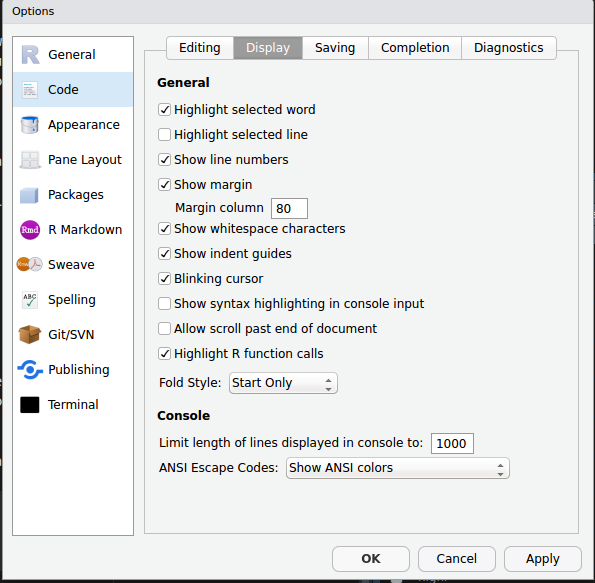
\includegraphics[width=0.5\linewidth]{options} 

}

\caption{Code display options}\label{fig:option-settings}
\end{figure}

\begin{itemize}
\tightlist
\item
  \emph{Highlight selected word}
\item
  \emph{Show line number}
\item
  \emph{Show margin} (and set margin column to 80)
\item
  \emph{Show whitespace characters}
\item
  \emph{Highlite R function calls}
\end{itemize}

Generally speaking those options, do not influence how your code is
performed, but will allow you to write cleaner and read easier. You can
also change colors of your environment in \emph{Appearance}.

\section{Installing packages}\label{installing-packages}

In your \emph{`Files'} winodow, you will find \emph{Packages} pane,
which contains \emph{Install} button. You can use it now, to install
packages needed to perform excercies from this book. The packages are:

\begin{figure}

{\centering 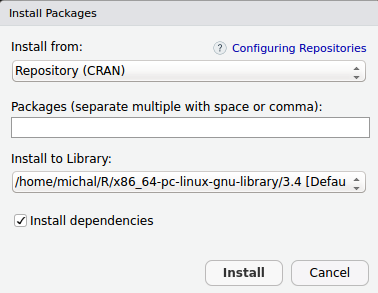
\includegraphics[width=0.5\linewidth]{instalPacks} 

}

\caption{Installation window}\label{fig:install-packs}
\end{figure}

\begin{itemize}
\tightlist
\item
  \textbf{devtools} \citep{R-devtools}
\item
  \textbf{tidyverse} \citep{R-dplyr}
\item
  \textbf{fitdistrplus} \citep{R-fitdistrplus}
\item
  \textbf{e1071} \citep{R-e1071}
\item
  \textbf{truncdist} \citep{R-truncdist}
\end{itemize}

Now everytime you need finctions from specyfic library you can just tick
box next to package name, and RStudio will load it for you.

\section{Conventions}\label{conventions}

In this book, we will use following conventions:

\begin{itemize}
\tightlist
\item
  Names of programs and packages are in \textbf{Bold}.
\item
  All other names e.g.~names of panes menu items as well as things that
  needs to be stressed are in \emph{italics}.
\item
  Function names and variables are always writen in inline code e.g.
  \texttt{t.test()} or \texttt{x}.
\item
  File names are wirten in inline code e.g. \texttt{foo.txt}.
\item
  Citations are in APA style, and `clickable' e.g.click on the name and
  year of \textbf{knitr} package citation \citep{xie2015}.
\item
  Code chunks are in blocks and result lines start with \#\#
\end{itemize}

\begin{Shaded}
\begin{Highlighting}[]
\KeywordTok{rnorm}\NormalTok{(}\DecValTok{10}\NormalTok{, }\DecValTok{1}\NormalTok{, }\FloatTok{0.5}\NormalTok{)}
\end{Highlighting}
\end{Shaded}

\begin{verbatim}
##  [1] 0.2569541 2.0800798 0.7579734 0.9364796 1.2213334 1.3123241 1.1047721
##  [8] 1.1495709 0.9991266 2.1900720
\end{verbatim}

\begin{itemize}
\tightlist
\item
  There are no \texttt{\textgreater{}} (\emph{prompt}) signs in code
  chunks.
\item
  Figures are floating - meaning, that they are not always imediately
  after they are mentioned in text.
\item
  Tables are in \emph{longtable} format (meaning they are not floating
  and might be multipage) e.g.
\end{itemize}

\begin{Shaded}
\begin{Highlighting}[]
\NormalTok{knitr}\OperatorTok{::}\KeywordTok{kable}\NormalTok{(}
  \KeywordTok{head}\NormalTok{(iris, }\DecValTok{25}\NormalTok{), }\DataTypeTok{caption =} \StringTok{'Example table'}\NormalTok{,}
  \DataTypeTok{booktabs =} \OtherTok{TRUE}\NormalTok{, }\DataTypeTok{longtable =} \OtherTok{TRUE}
\NormalTok{)}
\end{Highlighting}
\end{Shaded}

\begin{longtable}[t]{rrrrl}
\caption{\label{tab:nice-tab}Example table}\\
\toprule
Sepal.Length & Sepal.Width & Petal.Length & Petal.Width & Species\\
\midrule
5.1 & 3.5 & 1.4 & 0.2 & setosa\\
4.9 & 3.0 & 1.4 & 0.2 & setosa\\
4.7 & 3.2 & 1.3 & 0.2 & setosa\\
4.6 & 3.1 & 1.5 & 0.2 & setosa\\
5.0 & 3.6 & 1.4 & 0.2 & setosa\\
\addlinespace
5.4 & 3.9 & 1.7 & 0.4 & setosa\\
4.6 & 3.4 & 1.4 & 0.3 & setosa\\
5.0 & 3.4 & 1.5 & 0.2 & setosa\\
4.4 & 2.9 & 1.4 & 0.2 & setosa\\
4.9 & 3.1 & 1.5 & 0.1 & setosa\\
\addlinespace
5.4 & 3.7 & 1.5 & 0.2 & setosa\\
4.8 & 3.4 & 1.6 & 0.2 & setosa\\
4.8 & 3.0 & 1.4 & 0.1 & setosa\\
4.3 & 3.0 & 1.1 & 0.1 & setosa\\
5.8 & 4.0 & 1.2 & 0.2 & setosa\\
\addlinespace
5.7 & 4.4 & 1.5 & 0.4 & setosa\\
5.4 & 3.9 & 1.3 & 0.4 & setosa\\
5.1 & 3.5 & 1.4 & 0.3 & setosa\\
5.7 & 3.8 & 1.7 & 0.3 & setosa\\
5.1 & 3.8 & 1.5 & 0.3 & setosa\\
\addlinespace
5.4 & 3.4 & 1.7 & 0.2 & setosa\\
5.1 & 3.7 & 1.5 & 0.4 & setosa\\
4.6 & 3.6 & 1.0 & 0.2 & setosa\\
5.1 & 3.3 & 1.7 & 0.5 & setosa\\
4.8 & 3.4 & 1.9 & 0.2 & setosa\\
\bottomrule
\end{longtable}

\begin{itemize}
\tightlist
\item
  Tabels and figures are references are clickable e.g.~see Table
  \ref{tab:nice-tab} or see Figure \ref{fig:option-settings}.
\end{itemize}

\chapter{Basics}\label{basics}

\section{Getting started}\label{getting-started}

\subsection{Help}\label{help}

There are just few things you really need to remamber and follow when
you want to start using \textbf{R}. First, there is very good
\emph{help} build in. To access it, you use \texttt{?} sign with name of
function: eg: \texttt{?t.test}. After executing command, in your window
with \emph{Help} pane, a page dedicated to this function will pop up.
You will get information on syntax, options to use with this function
and in most caseses some code examples. However, with single question
mark you are telling \textbf{R} to only look into functions from
packages that are \emph{currently loaded} and have this \emph{precise
name}. If you want to tell \textbf{R} to look for proper function in
\emph{all packages} or you are not sure what the exact name is you can
use double question mark e.g. \texttt{??mutate}. In effect, in the same
pane and window as previously you will get a list of results that match
your query. Finally, using \emph{Packages} pane, you can click on one of
the packages names, to display all of the functions within it. Than by
clicking on the name of functions you are interested in, you will be
taken to proper page with description.

\subsection{Internet is a great source of
information}\label{internet-is-a-great-source-of-information}

Anytime you feel lost or need help that is beyond the scope of manuals,
just ask Google. For instance you can use this query: \emph{how to make
density plot in R}. Thanks to huge community you will find a lot of
answers. The most reliable ones can be found on \emph{StackOverflow},
\emph{StatsExchange} and \emph{RBloggers}. If you don't know if there is
a library to perform particular task also ask uncle Google. For instace,
if you want to use random numbers from Dirichlet distribution, you can
use this query: \emph{dirichlet distribution r}.

\subsection{More on internet sources}\label{more-on-internet-sources}

A good practice, when you want to learn programming language is to read
what other people do and how the code. In the begginig it might be a bit
overwhealming or confusing to read all the stuff. However, reading
others work will get you used to syntax and workflow, and will qive you
great basics to invent your own code. Hopefuly, you don't need to spend
hours for searching some interesting blogs. There is great blog
agregator \href{https://rweekly.org}{R weekly} that gathers in one place
best posts, podcasts, etc. on \textbf{R}, every week.

\section{Syntax}\label{syntax}

\subsection{Common operators}\label{common-operators}

There are three main \emph{signs} used in \textbf{R's} syntax. First two
are assigment symbols: \texttt{\textless{}-} and to \texttt{=}; for
convention we use them in different cases. Third one is \texttt{\#}. It
is a symbol used for comments. Everything following this symbol to the
end of code line will not be executed. There are also other signs (or
symbols) which are building blocks of language, however their use is
very precisely defined and reserved for certain events. Below you find a
table with reference for most common operators used. You will faster
grasp it while you write your own code, than by reading about it. Thus,
I suggest we go deeper into variable types in \textbf{R} language.

\begin{longtable}[t]{lll}
\caption{\label{tab:tab-operators}Common operators in R}\\
\toprule
sign & type & action\\
\midrule
+ & maths & addition\\
- & maths & substraction\\
* & maths & multiplication\\
/ & maths & division\\
\%\% & maths & modulo\\
\addlinespace
\textasciicircum{} & maths & power\\
> & relations & left greater\\
>= & relations & left greater of equal\\
< & relations & right greater\\
<= & relations & right greater or equal\\
\addlinespace
== & relations & left equal right\\
!= & relations & left uneqal right\\
! & logics & not\\
\& & logics & and\\
| & logics & or\\
\addlinespace
\textasciitilde{} & model & left relates to right\\
<- or -> & assignment & assignes value to variable\\
\$ & address & extracts values with 'element name' from variable\\
: & sequence & creates sequence of numbers from 'left value' to 'right value'\\
\%>\% or \%<>\% & piping & pipes results(from left) as arguments to functionon right\\
\bottomrule
\end{longtable}

\subsection{Variables}\label{variables}

Concept of variable is crucial for programming. In \textbf{R} variables
can contain many things: vectors, data frames, results of statistical
analyses etc. Each of variables have some characteristic properties.
They are defined by \emph{class} of the variable. Thanks to \emph{class}
atribute, \textbf{R} knows, how to deal with variable -- what is the
internal structure and what operations can be performed over variable.
Data can be stored in variables in different manners. To assign
something to variable we use \texttt{\textless{}-} operator, which tells
\textbf{R} to store right side of arrow under name on the left side of
arrow. The simplest variable is \emph{vector}, which can be of
\emph{class}: \emph{character}, \emph{integer}, \emph{numeric} or
\emph{logical}. For instance:

\begin{Shaded}
\begin{Highlighting}[]
\NormalTok{characterVector <-}\StringTok{ }\KeywordTok{c}\NormalTok{(}\StringTok{'a'}\NormalTok{, }\StringTok{'b'}\NormalTok{, }\StringTok{'c'}\NormalTok{)}
\KeywordTok{class}\NormalTok{(characterVector)}
\end{Highlighting}
\end{Shaded}

\begin{verbatim}
## [1] "character"
\end{verbatim}

\begin{Shaded}
\begin{Highlighting}[]
\NormalTok{integerVector <-}\StringTok{ }\KeywordTok{c}\NormalTok{(1L, 2L, 3L)}
\KeywordTok{class}\NormalTok{(integerVector)}
\end{Highlighting}
\end{Shaded}

\begin{verbatim}
## [1] "integer"
\end{verbatim}

\begin{Shaded}
\begin{Highlighting}[]
\NormalTok{numericVector <-}\StringTok{ }\KeywordTok{c}\NormalTok{(}\FloatTok{2.5}\NormalTok{, }\FloatTok{3.5}\NormalTok{, }\FloatTok{4.5}\NormalTok{)}
\KeywordTok{class}\NormalTok{(numericVector)}
\end{Highlighting}
\end{Shaded}

\begin{verbatim}
## [1] "numeric"
\end{verbatim}

\begin{Shaded}
\begin{Highlighting}[]
\NormalTok{logicalVector <-}\StringTok{ }\KeywordTok{c}\NormalTok{(}\OtherTok{TRUE}\NormalTok{, }\OtherTok{FALSE}\NormalTok{)}
\KeywordTok{class}\NormalTok{(logicalVector)}
\end{Highlighting}
\end{Shaded}

\begin{verbatim}
## [1] "logical"
\end{verbatim}

For more complex data, we have three basic classes: \emph{lists},
\emph{data frames} and \emph{matrices}. \emph{Matrix} is simillar to
\emph{data frame}. The most obvious difference is that \emph{matrix}
contains only one \emph{class} of variables (usually \emph{numeric} or
\emph{integer}), while \emph{data frame} can store \emph{numeric}, as
well as \emph{characters} and \emph{factors} (for now, you can assume
that \emph{factor} class is used to store catagorical variables) in
seprate columns. Also \emph{matrices} are used when programmers want to
achive great speed in mathematical computation. \emph{Data frames} are
resembling tables from popular spreadsheet software. Lets look:

\begin{Shaded}
\begin{Highlighting}[]
\NormalTok{matrixVariable <-}\StringTok{ }\KeywordTok{matrix}\NormalTok{(}\KeywordTok{c}\NormalTok{(}\DecValTok{1}\OperatorTok{:}\DecValTok{10}\NormalTok{), }\DataTypeTok{nrow =} \DecValTok{2}\NormalTok{)}
\NormalTok{matrixVariable}
\end{Highlighting}
\end{Shaded}

\begin{verbatim}
##      [,1] [,2] [,3] [,4] [,5]
## [1,]    1    3    5    7    9
## [2,]    2    4    6    8   10
\end{verbatim}

\begin{Shaded}
\begin{Highlighting}[]
\KeywordTok{class}\NormalTok{(matrixVariable)}
\end{Highlighting}
\end{Shaded}

\begin{verbatim}
## [1] "matrix"
\end{verbatim}

\begin{Shaded}
\begin{Highlighting}[]
\NormalTok{dfVariable <-}\StringTok{ }\KeywordTok{data.frame}\NormalTok{(}\DataTypeTok{x1 =} \DecValTok{1}\OperatorTok{:}\DecValTok{5}\NormalTok{, }\DataTypeTok{x2 =} \DecValTok{6}\OperatorTok{:}\DecValTok{10}\NormalTok{)}
\NormalTok{dfVariable}
\end{Highlighting}
\end{Shaded}

\begin{verbatim}
##   x1 x2
## 1  1  6
## 2  2  7
## 3  3  8
## 4  4  9
## 5  5 10
\end{verbatim}

\begin{Shaded}
\begin{Highlighting}[]
\KeywordTok{class}\NormalTok{(dfVariable)}
\end{Highlighting}
\end{Shaded}

\begin{verbatim}
## [1] "data.frame"
\end{verbatim}

\emph{Lists} are\ldots{} lists of variables. Each \emph{list} element
can be of different \emph{class} and length. To grasp the idea of
\emph{lists} it will be best to present it with example:

\begin{Shaded}
\begin{Highlighting}[]
\NormalTok{listVariable <-}\StringTok{ }\KeywordTok{list}\NormalTok{(}\DataTypeTok{x1 =} \KeywordTok{c}\NormalTok{(}\StringTok{"a"}\NormalTok{, }\StringTok{"b"}\NormalTok{), }\DataTypeTok{x2 =} \DecValTok{1}\OperatorTok{:}\DecValTok{4}\NormalTok{, }\DataTypeTok{x3 =} \KeywordTok{matrix}\NormalTok{(}\KeywordTok{c}\NormalTok{(}\DecValTok{1}\OperatorTok{:}\DecValTok{6}\NormalTok{), }\DataTypeTok{nrow =} \DecValTok{2}\NormalTok{))}
\NormalTok{listVariable}
\end{Highlighting}
\end{Shaded}

\begin{verbatim}
## $x1
## [1] "a" "b"
## 
## $x2
## [1] 1 2 3 4
## 
## $x3
##      [,1] [,2] [,3]
## [1,]    1    3    5
## [2,]    2    4    6
\end{verbatim}

\begin{Shaded}
\begin{Highlighting}[]
\KeywordTok{class}\NormalTok{(listVariable)}
\end{Highlighting}
\end{Shaded}

\begin{verbatim}
## [1] "list"
\end{verbatim}

\begin{Shaded}
\begin{Highlighting}[]
\KeywordTok{class}\NormalTok{(listVariable}\OperatorTok{$}\NormalTok{x1)}
\end{Highlighting}
\end{Shaded}

\begin{verbatim}
## [1] "character"
\end{verbatim}

\begin{Shaded}
\begin{Highlighting}[]
\KeywordTok{class}\NormalTok{(listVariable}\OperatorTok{$}\NormalTok{x2)}
\end{Highlighting}
\end{Shaded}

\begin{verbatim}
## [1] "integer"
\end{verbatim}

\begin{Shaded}
\begin{Highlighting}[]
\KeywordTok{class}\NormalTok{(listVariable}\OperatorTok{$}\NormalTok{x3)}
\end{Highlighting}
\end{Shaded}

\begin{verbatim}
## [1] "matrix"
\end{verbatim}

There are plenty of other \emph{classes}, e.g.~for \emph{time
variables}, however mentioned above are the basic ones you will deal
mostly. Also because they are so often used, you should learn how to
recognize their structure at a glance. Later on, I will present you how
(and when) each of this variables types can be used in work.

\subsection{Naming Variables}\label{naming-variables}

First of all all names are \emph{case-sensitive}, which means that
\textbf{R} recognize variables named \texttt{RVariable},
\texttt{rVariable} and \texttt{Rvariable} as three different objects.
Second thing to remamber is that variable name \emph{have to} start with
a letter and may contain only letters, numbers and symbols: . (dot) and
\_ (underscore). There are also some \emph{good practices} in naming
variables (after \href{http://adv-r.had.com.nz/Style.html}{Hadley
Wickham Style guide}):

\begin{itemize}
\tightlist
\item
  use lowercase to names variables (and functions)
\item
  use nouns to name variables (and verbs for functions)
\item
  try to be precise when naming
\item
  try to be concise when naming
\item
  use underscore \_ to separate words (snake\_case) e.g.
  \texttt{first\_variable}
\item
  \emph{some other guidelines suggest using camel cases e.g.}
  \texttt{firstVariable}
\end{itemize}

And the golden rule should be - whatever guideline you follow -- be
consequent!

\subsection{Math operations}\label{math-operations}

In \textbf{R} we use standard math oprators \texttt{+\ -\ *\ /} to
perform addition, substraction, multiplication and division. Symbol
\texttt{\^{}} indicates that we want to use power, and sqrt to make
square root. Ok, so whats the name of a function to get
n\textsuperscript{th} root? Probably you remamber from math lessons that
\(\sqrt [n] {x} = x^\frac{1}{n}\), thus you can just write
\texttt{x\^{}(1/n)}. To change order of operation (which are following
mathematics rules) use brackets \texttt{()}. Other important
mathematical functions are \texttt{\%\%} for modulo, and \%/\% for
integer division.

\begin{Shaded}
\begin{Highlighting}[]
\DecValTok{5} \OperatorTok{+}\StringTok{ }\DecValTok{2}
\end{Highlighting}
\end{Shaded}

\begin{verbatim}
## [1] 7
\end{verbatim}

\begin{Shaded}
\begin{Highlighting}[]
\DecValTok{11} \OperatorTok{-}\StringTok{ }\DecValTok{3}
\end{Highlighting}
\end{Shaded}

\begin{verbatim}
## [1] 8
\end{verbatim}

\begin{Shaded}
\begin{Highlighting}[]
\NormalTok{(}\DecValTok{4}\OperatorTok{+}\DecValTok{7}\NormalTok{)}\OperatorTok{/}\DecValTok{9}\OperatorTok{*}\DecValTok{2}
\end{Highlighting}
\end{Shaded}

\begin{verbatim}
## [1] 2.444444
\end{verbatim}

\begin{Shaded}
\begin{Highlighting}[]
\DecValTok{14} \OperatorTok\StringTok{ }\DecValTok{3} \OperatorTok{+}\StringTok{ }\DecValTok{1}
\end{Highlighting}
\end{Shaded}

\begin{verbatim}
## [1] 5
\end{verbatim}

\begin{Shaded}
\begin{Highlighting}[]
\DecValTok{8}\OperatorTok{^}\NormalTok{(}\DecValTok{1}\OperatorTok{/}\DecValTok{3}\NormalTok{) }\OperatorTok{+}\StringTok{ }\DecValTok{10}\OperatorTok\DecValTok{6}
\end{Highlighting}
\end{Shaded}

\begin{verbatim}
## [1] 6
\end{verbatim}

To calculate logarithms there is \emph{build in} function
\texttt{log()}. It uses as a base Eulers number by default, however you
can override it i.e. \texttt{log(10,\ base\ =\ 10)}. You can calculate
exponential function using \texttt{exp()} function. There are also
trigonometric functions in \textbf{R}: \texttt{sin()}, \texttt{cos()},
\texttt{tan()}, \texttt{asin()}, \texttt{acos()}, \texttt{atan()}.
Angles are used/expressed in radians. To transform values from degrees
to radians multiply by \texttt{pi} and divide by 180. To transform
values from radians to degrees multiply by 180 and divide by
\texttt{pi}. By the way, \texttt{pi} is a constant in \textbf{R},
meaning that its value is build in the language (simmliar as Euler
number is \texttt{exp(1)}).

\begin{Shaded}
\begin{Highlighting}[]
\NormalTok{someArc <-}\StringTok{ }\DecValTok{90}\OperatorTok{*}\NormalTok{pi}\OperatorTok{/}\DecValTok{180}
\KeywordTok{sin}\NormalTok{(someArc)}
\end{Highlighting}
\end{Shaded}

\begin{verbatim}
## [1] 1
\end{verbatim}

\begin{Shaded}
\begin{Highlighting}[]
\NormalTok{atanValue <-}\StringTok{ }\KeywordTok{atan}\NormalTok{(}\FloatTok{0.89}\NormalTok{)}
\NormalTok{atanValue}\OperatorTok{*}\DecValTok{180}\OperatorTok{/}\NormalTok{pi}
\end{Highlighting}
\end{Shaded}

\begin{verbatim}
## [1] 41.66908
\end{verbatim}

\subsection{Logics}\label{logics}

Logical expression are often used in programming. They compare left side
with right side arguments of statement. The result of those comparrision
might be \texttt{TRUE} or \texttt{FALSE} (in many other languages those
are called \emph{Boolean} values) which belong to \emph{class Logical}.
In Table \ref{tab:tab-operators} you will find list of most common
logical operarators used to build statements. Here is a small
\emph{cheatsheet tables}:

\begin{table}

\begin{longtable}[t]{llll}
\toprule
  & NA & FALSE & TRUE\\
\midrule
NA & NA & FALSE & NA\\
FALSE & FALSE & FALSE & FALSE\\
TRUE & NA & FALSE & TRUE\\
\bottomrule
\end{longtable}
\begin{longtable}[t]{llll}
\toprule
  & NA & FALSE & TRUE\\
\midrule
NA & NA & NA & TRUE\\
FALSE & NA & FALSE & TRUE\\
TRUE & TRUE & TRUE & TRUE\\
\bottomrule
\end{longtable}
\end{table}

Below you can see them in action:

\begin{Shaded}
\begin{Highlighting}[]
\DecValTok{5} \OperatorTok{>=}\StringTok{ }\DecValTok{1}
\end{Highlighting}
\end{Shaded}

\begin{verbatim}
## [1] TRUE
\end{verbatim}

\begin{Shaded}
\begin{Highlighting}[]
\DecValTok{10}\OperatorTok\DecValTok{2} \OperatorTok{==}\StringTok{ }\DecValTok{0}
\end{Highlighting}
\end{Shaded}

\begin{verbatim}
## [1] TRUE
\end{verbatim}

\begin{Shaded}
\begin{Highlighting}[]
\OperatorTok{!}\OtherTok{FALSE}
\end{Highlighting}
\end{Shaded}

\begin{verbatim}
## [1] TRUE
\end{verbatim}

\begin{Shaded}
\begin{Highlighting}[]
\NormalTok{5L }\OperatorTok{|}\StringTok{ }\FloatTok{11.1} \OperatorTok{<=}\StringTok{ }\DecValTok{6}
\end{Highlighting}
\end{Shaded}

\begin{verbatim}
## [1] TRUE
\end{verbatim}

\subsection{Functions}\label{functions}

When writing code we generally want to perform some actions on our
variables. There is a lot of \emph{build in functions} in base
\textbf{R} distribution, and a whole Galaxy of \emph{functions} provided
by community. Function can be literally any action performed on
variables. For instance, there are some build in statistical functions
like \texttt{t.test()} or \texttt{chisq.test()}. Other function can be
use to draw some charts and plots, e.g. \texttt{plot()}. It's easy to
recognize function, since its structere is \emph{name} follwoed by
parentheses \emph{()}. Inside parentheses user provides arguments and
options to function. Lests see how it works with one of \emph{build in}
functions:

\begin{Shaded}
\begin{Highlighting}[]
\NormalTok{tTestResult <-}\StringTok{ }\KeywordTok{t.test}\NormalTok{(numericVector, integerVector)}
\KeywordTok{print}\NormalTok{(tTestResult)}
\end{Highlighting}
\end{Shaded}

\begin{verbatim}
## 
##  Welch Two Sample t-test
## 
## data:  numericVector and integerVector
## t = 1.8371, df = 4, p-value = 0.1401
## alternative hypothesis: true difference in means is not equal to 0
## 95 percent confidence interval:
##  -0.7669579  3.7669579
## sample estimates:
## mean of x mean of y 
##       3.5       2.0
\end{verbatim}

We used \texttt{t.test()} function, with two arguments:
\texttt{numericVector} and \texttt{integerVector}. In second function
call, we \emph{ordered} \textbf{R} to print out the results of
statistical test stored in variable \texttt{tTestResult} -- which is the
argument of this function.

\chapter{Somwehere between basic and
useful}\label{somwehere-between-basic-and-useful}

\section{Addressing}\label{addressing}

\subsection{Vectors}\label{vectors}

When you deal with variables you often will want to use only a part of
it in your work. Other times you will want to get rid of some values
which follow certain criteria. In order to do it you need to know an
`addrress' of particular value in a \emph{vector}, \emph{data frame},
\emph{list} etc. From now on, I will use some functions while describing
it \emph{at hoc}, since I believe the best way to learn them, is to use
them. Lets creat a \emph{vector} and see what we can do with it.

\begin{Shaded}
\begin{Highlighting}[]
\NormalTok{addressVec <-}\StringTok{ }\KeywordTok{seq}\NormalTok{(}\DataTypeTok{from =} \DecValTok{1}\NormalTok{, }\DataTypeTok{to =} \DecValTok{20}\NormalTok{, }\DataTypeTok{by =} \DecValTok{2}\NormalTok{)}
\NormalTok{addressVec}
\end{Highlighting}
\end{Shaded}

\begin{verbatim}
##  [1]  1  3  5  7  9 11 13 15 17 19
\end{verbatim}

Instead of typing all the numbers by hand, we can use \texttt{seq()}
function, to generate it automatically. This function takes two
arguments \texttt{from} and \texttt{to}, however additionaly we can use
option \texttt{by} which defines increment of the sequence. As your
knowledge is growing I can tell you a secret. Often there is no need to
name all the arguments and options in functions body. In the beginning
you should use the names, but the more experienced you get you will
notice that you omit them often. Actually we nearly always omit so
called \emph{default} options of a function. Use \texttt{?seq} to check
the help page for this function. You will see that it can take more
options than \texttt{from}, \texttt{to} and \texttt{by}, but since they
are predifned we don't neet to bother and type them as long as we are OK
with \emph{default} settings. So, lets retype our \emph{variable}
definition:

\begin{Shaded}
\begin{Highlighting}[]
\NormalTok{addressVec <-}\StringTok{ }\KeywordTok{seq}\NormalTok{(}\DecValTok{1}\NormalTok{, }\DecValTok{20}\NormalTok{, }\DecValTok{2}\NormalTok{)}
\NormalTok{addressVec}
\end{Highlighting}
\end{Shaded}

\begin{verbatim}
##  [1]  1  3  5  7  9 11 13 15 17 19
\end{verbatim}

The results are identical. Lets get back to addressing issues. Suppose
you want to check the fifth element of a our \texttt{addressVec}
variable. To do it we use variable name followed by element number in
brackets (or square brakcets, if you will).

\begin{Shaded}
\begin{Highlighting}[]
\NormalTok{addressVec[}\DecValTok{5}\NormalTok{]}
\end{Highlighting}
\end{Shaded}

\begin{verbatim}
## [1] 9
\end{verbatim}

If you want to get rid of fifth element just preced it with -.

\begin{Shaded}
\begin{Highlighting}[]
\NormalTok{addressVec[}\OperatorTok{-}\DecValTok{5}\NormalTok{]}
\end{Highlighting}
\end{Shaded}

\begin{verbatim}
## [1]  1  3  5  7 11 13 15 17 19
\end{verbatim}

Easy. The thing that is worth to mention right now is that \textbf{R
Core Team} have reason and dignity of human beings so they start
numeration of elements with value 1. In some other languages, because of
no sensible reasons numeration starts with 0 -- which is horribly
annoing. What to do if we want to extract values of more than one
element?

\begin{Shaded}
\begin{Highlighting}[]
\NormalTok{addressVec[}\DecValTok{1}\NormalTok{,}\DecValTok{5}\NormalTok{]}
\end{Highlighting}
\end{Shaded}

\begin{verbatim}
## Error in addressVec[1, 5]: incorrect number of dimensions
\end{verbatim}

\begin{Shaded}
\begin{Highlighting}[]
\NormalTok{addressVec[}\OperatorTok{-}\DecValTok{1}\NormalTok{,}\OperatorTok{-}\DecValTok{5}\NormalTok{,}\OperatorTok{-}\DecValTok{6}\NormalTok{]}
\end{Highlighting}
\end{Shaded}

\begin{verbatim}
## Error in addressVec[-1, -5, -6]: incorrect number of dimensions
\end{verbatim}

Error occurs with warning that there is incorrect number of dimensions.
That's because \emph{vectors} have only one dimension -- length. Within
square brackets comma separates dimensions. So when we used command
\texttt{{[}1,5{]}} we told R to look for value that address is number 1
in first dimension and number 5 in second dimension. To correct the
mistake, we need to provide a vector of numbers from first dimension. We
can use \texttt{c()} function to create \emph{ad hoc} \emph{vector}
inside square brackets.

\begin{Shaded}
\begin{Highlighting}[]
\NormalTok{addressVec[}\KeywordTok{c}\NormalTok{(}\DecValTok{1}\NormalTok{,}\DecValTok{5}\NormalTok{)]}
\end{Highlighting}
\end{Shaded}

\begin{verbatim}
## [1] 1 9
\end{verbatim}

\begin{Shaded}
\begin{Highlighting}[]
\NormalTok{addressVec[}\OperatorTok{-}\KeywordTok{c}\NormalTok{(}\DecValTok{1}\NormalTok{,}\DecValTok{5}\NormalTok{,}\DecValTok{6}\NormalTok{)]}
\end{Highlighting}
\end{Shaded}

\begin{verbatim}
## [1]  3  5  7 13 15 17 19
\end{verbatim}

Now something more complicated. Try to figure out what code below does,
and what is the result of \texttt{which()} function:

\begin{Shaded}
\begin{Highlighting}[]
\NormalTok{addressVec[}\KeywordTok{which}\NormalTok{(addressVec }\OperatorTok{>=}\StringTok{ }\DecValTok{6}\NormalTok{)] <-}\StringTok{ 'o..O'}
\NormalTok{addressVec}
\end{Highlighting}
\end{Shaded}

\begin{verbatim}
##  [1] "1"    "3"    "5"    "o..O" "o..O" "o..O" "o..O" "o..O" "o..O" "o..O"
\end{verbatim}

If you have problems, you can think of this example as a composition of
actions. First there is expression
\texttt{addressVec\ \textgreater{}=6}, than we use \texttt{which()}
function with argument from previous expression. Next the result is
passed as an address. Last thing is assigment of new value to\ldots{}

\subsection{Data frames (and matrices)}\label{data-frames-and-matrices}

When dealing with \emph{data frames} and addressing is possible in two
ways. First is simmilar to \emph{vector} addressing. However, as
\emph{data frames} have two dimentions, you will need to express them
like \texttt{df{[}1,2{]}} -- which tells \textbf{R} to look up the cell
in row 1, column 2. But what if you want to check all the cells in
particular row or column? Omit the number, but not the coma -- like
this: \texttt{df{[},3{]}}. It will display all row values from column 3.
And of course you can still use \emph{vectors} when addressing. This way
is also working for \emph{matrices}.

\begin{Shaded}
\begin{Highlighting}[]
\NormalTok{addressDF <-}\StringTok{ }\KeywordTok{data.frame}\NormalTok{(}\DataTypeTok{C1 =} \KeywordTok{seq}\NormalTok{(}\DecValTok{1}\NormalTok{,}\DecValTok{10}\NormalTok{), }\DataTypeTok{C2 =} \KeywordTok{seq}\NormalTok{(}\DecValTok{11}\NormalTok{,}\DecValTok{20}\NormalTok{), }\DataTypeTok{C3 =} \KeywordTok{seq}\NormalTok{(}\DecValTok{21}\NormalTok{,}\DecValTok{30}\NormalTok{))}
\NormalTok{addressDF[}\DecValTok{5}\NormalTok{,}\DecValTok{2}\NormalTok{]}
\end{Highlighting}
\end{Shaded}

\begin{verbatim}
## [1] 15
\end{verbatim}

\begin{Shaded}
\begin{Highlighting}[]
\NormalTok{addressDF[}\DecValTok{6}\NormalTok{,]}
\end{Highlighting}
\end{Shaded}

\begin{verbatim}
##   C1 C2 C3
## 6  6 16 26
\end{verbatim}

\begin{Shaded}
\begin{Highlighting}[]
\NormalTok{addressDF[}\KeywordTok{c}\NormalTok{(}\DecValTok{6}\NormalTok{,}\DecValTok{7}\NormalTok{), }\DecValTok{1}\OperatorTok{:}\DecValTok{3}\NormalTok{]}
\end{Highlighting}
\end{Shaded}

\begin{verbatim}
##   C1 C2 C3
## 6  6 16 26
## 7  7 17 27
\end{verbatim}

The second option is tu use \texttt{\$} sign followed with column name
(and it work only for \emph{data frames} and \emph{lists}). This way, we
tell \textbf{R} to look in whole column. If we want to display values
from particular cells, we put them in brackets after column name, the
same way as we do for \emph{vectors}:

\begin{Shaded}
\begin{Highlighting}[]
\NormalTok{addressDF}\OperatorTok{$}\NormalTok{C2[}\DecValTok{5}\NormalTok{]}
\end{Highlighting}
\end{Shaded}

\begin{verbatim}
## [1] 15
\end{verbatim}

\begin{Shaded}
\begin{Highlighting}[]
\NormalTok{addressDF}\OperatorTok{$}\NormalTok{C3[}\KeywordTok{c}\NormalTok{(}\DecValTok{6}\OperatorTok{:}\DecValTok{9}\NormalTok{)]}
\end{Highlighting}
\end{Shaded}

\begin{verbatim}
## [1] 26 27 28 29
\end{verbatim}

\subsection{Lists}\label{lists}

As mentioned before each \emph{list} element can have different
structure. Thus, addressing is kind of a mixture of all above. First you
need to address element of your \emph{list}. You do it with double
brakcets containing element number following name of variable. You can
also use \texttt{\$} sign with name of the element. Than you use
addressing the same way you address \emph{data frames}, \emph{vectors}
or \emph{matrices}.

\begin{Shaded}
\begin{Highlighting}[]
\NormalTok{addressList <-}\StringTok{ }\KeywordTok{list}\NormalTok{(}\DataTypeTok{x1 =} \KeywordTok{c}\NormalTok{(}\StringTok{'a'}\NormalTok{, }\StringTok{'b'}\NormalTok{), }\DataTypeTok{x2 =} \DecValTok{1}\OperatorTok{:}\DecValTok{4}\NormalTok{, }\DataTypeTok{x3 =} \KeywordTok{matrix}\NormalTok{(}\KeywordTok{c}\NormalTok{(}\DecValTok{1}\OperatorTok{:}\DecValTok{6}\NormalTok{), }\DataTypeTok{nrow =} \DecValTok{2}\NormalTok{))}
\NormalTok{addressList[[}\DecValTok{2}\NormalTok{]]}
\end{Highlighting}
\end{Shaded}

\begin{verbatim}
## [1] 1 2 3 4
\end{verbatim}

\begin{Shaded}
\begin{Highlighting}[]
\NormalTok{addressList}\OperatorTok{$}\NormalTok{x2[}\DecValTok{3}\NormalTok{]}
\end{Highlighting}
\end{Shaded}

\begin{verbatim}
## [1] 3
\end{verbatim}

\begin{Shaded}
\begin{Highlighting}[]
\NormalTok{addressList[[}\DecValTok{3}\NormalTok{]]}
\end{Highlighting}
\end{Shaded}

\begin{verbatim}
##      [,1] [,2] [,3]
## [1,]    1    3    5
## [2,]    2    4    6
\end{verbatim}

\begin{Shaded}
\begin{Highlighting}[]
\NormalTok{addressList[[}\DecValTok{3}\NormalTok{]][,}\DecValTok{3}\NormalTok{]}
\end{Highlighting}
\end{Shaded}

\begin{verbatim}
## [1] 5 6
\end{verbatim}

Ok, now simple task for you. There is a function called
\texttt{colnames()} which allow us to change names in \emph{matrix}
variable. To use it you need to put name of \emph{matrix} variable in
the parentheses (like this: \texttt{colnames(x)}), and assign value to
it (e.g.
\texttt{colnames(x)\ \textless{}-\ c(\textquotesingle{}one\textquotesingle{},\ \textquotesingle{}two\textquotesingle{})).\ Now\ change\ names\ of\ of\ columns\ in\ *matrix*\ that\ is\ element\ of\ list\ above\ to}I`,
`Love', `R'.

\section{Operation on Vectors}\label{operation-on-vectors}

Old proverb:

\begin{quote}
\emph{The power of R is vectorization}
\end{quote}

Indeed, vectorization is one of the most usefull features of \textbf{R}
environment. In short words, many functions are contructued in such
manner that one can avoid using loops (since, they are often very slow).
When you begin your journey with programming you will probably not
notice the difference in computation speed between \emph{vectorized way}
and \emph{loop way}. Nonetheless, what will you find attractive, is that
in many cases writting in vectorized form feels more natural. So how it
works? Most basic functions are \emph{written and compiled} in very
fast, low level languages like \textbf{C} or \textbf{FORTRAN}. It makes
computation way faster, but still we use easy \textbf{R} syntax. Instead
of running the \emph{precompiled} function on each of the elements of
vector we actually can pass the vector into function -- and \textbf{R}
will know what to do. The speed is achieved beacause when we use
function on each element, \textbf{R} needs to figure out what to do
several (or even hundred or thousands of) times, however when we pass
whole vector into function, it needs to find out what to do only once.
Sometimes, however we need to use some other functions, wich are not
meant to process vectors (or you want to use some arbitrary functions on
matrix, data frame or list). You will need to parse your data more than
once to function. In \textbf{R} you can do it by using loops or by using
so called \texttt{apply} family functions. When I was learning
\textbf{R} it was most confusing thing to me, however once you get it,
they become fairly easy to use. The most important difference for you as
a beginer is that when using loops you should make some memory
allocation -- in human language, before you run loop, you should create
vector which will store results. The loops achieve highest speed when
your vector can fit all the values from loop. If you do not know how big
your vector will be, you need to relay on \textbf{R} ability to
re-allocate the memory, which is \textbf{S L O W}. \texttt{apply} family
hopefully takes care of this problem, so everytime you know how to --
use it. It will save you time and frustration of using loops. I will
cover basic use of this functions later on examples.

\section{Randomization and
distribution}\label{randomization-and-distribution}

Random sampling is quite easy task. There is nice \texttt{sample()}
function, that allow you to do that. You can sample from \emph{numeric},
\emph{integer} or even \emph{character} \emph{vectors}. You can even
assign probabilities to particular elements of vector (we will not need
that at the moment). So lets make some fun and make virtual casino. We
will take two dice and will roll it 1000 times. If the sum of each
result is greater odd and smaller than \texttt{5} we will earn 30EUR. If
it is odd and higher than \texttt{5}, we will get 50EUR. However if the
sum is even number we loose 70EUR. Lets see if we can beat
casino\ldots{} First lets define our dice and rolls.

\begin{Shaded}
\begin{Highlighting}[]
\NormalTok{niceDice <-}\StringTok{ }\KeywordTok{seq}\NormalTok{(}\DecValTok{1}\NormalTok{,}\DecValTok{6}\NormalTok{)}
\NormalTok{rollDiceOne <-}\StringTok{ }\KeywordTok{sample}\NormalTok{(niceDice, }\DecValTok{1000}\NormalTok{, }\DataTypeTok{replace =}\NormalTok{ T)}
\NormalTok{rollDiceTwo <-}\StringTok{ }\KeywordTok{sample}\NormalTok{(niceDice, }\DecValTok{1000}\NormalTok{, }\DataTypeTok{replace =}\NormalTok{ T)}
\end{Highlighting}
\end{Shaded}

Ok, you heard about power of vectorization, already so lets sum up both
vectors:

\begin{Shaded}
\begin{Highlighting}[]
\NormalTok{sumDiceRolls <-}\StringTok{ }\NormalTok{rollDiceOne }\OperatorTok{+}\StringTok{ }\NormalTok{rollDiceTwo}
\end{Highlighting}
\end{Shaded}

Next lets make some use of knowledge we have already and subsitute our
results with some cash\ldots{}

\begin{Shaded}
\begin{Highlighting}[]
\NormalTok{cashDiceRolls <-}\StringTok{ }\NormalTok{sumDiceRolls}
\NormalTok{cashDiceRolls[}\KeywordTok{which}\NormalTok{(cashDiceRolls }\OperatorTok\StringTok{ }\DecValTok{2} \OperatorTok{==}\StringTok{ }\DecValTok{1} \OperatorTok{&}\StringTok{ }\NormalTok{cashDiceRolls }\OperatorTok{<=}\StringTok{ }\DecValTok{5}\NormalTok{)] <-}\StringTok{ }\DecValTok{30}
\NormalTok{cashDiceRolls[}\KeywordTok{which}\NormalTok{(cashDiceRolls }\OperatorTok\StringTok{ }\DecValTok{2} \OperatorTok{==}\StringTok{ }\DecValTok{1} \OperatorTok{&}\StringTok{ }\NormalTok{cashDiceRolls }\OperatorTok{>}\StringTok{ }\DecValTok{5}\NormalTok{)] <-}\StringTok{ }\DecValTok{50}
\NormalTok{cashDiceRolls[}\KeywordTok{which}\NormalTok{(cashDiceRolls }\OperatorTok\StringTok{ }\DecValTok{2} \OperatorTok{==}\StringTok{ }\DecValTok{0}\NormalTok{)] <-}\StringTok{ }\OperatorTok{-}\DecValTok{70}
\KeywordTok{sum}\NormalTok{(cashDiceRolls)}
\end{Highlighting}
\end{Shaded}

\begin{verbatim}
## [1] -70000
\end{verbatim}

Ok. What happened? We put our substitutoons in very wrong order\ldots{}
After first two substitutions we have only even numbers in our
vector\ldots{} So how to fix it? Start with assigning the highghest
absolute value, and after all change it to negative one.

\begin{Shaded}
\begin{Highlighting}[]
\NormalTok{cashDiceRolls <-}\StringTok{ }\NormalTok{sumDiceRolls}
\NormalTok{cashDiceRolls[}\KeywordTok{which}\NormalTok{(cashDiceRolls }\OperatorTok\StringTok{ }\DecValTok{2} \OperatorTok{==}\StringTok{ }\DecValTok{0}\NormalTok{)] <-}\StringTok{ }\DecValTok{70}
\NormalTok{cashDiceRolls[}\KeywordTok{which}\NormalTok{(cashDiceRolls }\OperatorTok\StringTok{ }\DecValTok{2} \OperatorTok{==}\StringTok{ }\DecValTok{1} \OperatorTok{&}\StringTok{ }\NormalTok{cashDiceRolls }\OperatorTok{>}\StringTok{ }\DecValTok{5}\NormalTok{)] <-}\StringTok{ }\DecValTok{50}
\NormalTok{cashDiceRolls[}\KeywordTok{which}\NormalTok{(cashDiceRolls }\OperatorTok\StringTok{ }\DecValTok{2} \OperatorTok{==}\StringTok{ }\DecValTok{1} \OperatorTok{&}\StringTok{ }\NormalTok{cashDiceRolls }\OperatorTok{<=}\StringTok{ }\DecValTok{5}\NormalTok{)] <-}\StringTok{ }\DecValTok{30}
\NormalTok{cashDiceRolls[}\KeywordTok{which}\NormalTok{(cashDiceRolls  }\OperatorTok{==}\StringTok{ }\DecValTok{70}\NormalTok{)] <-}\StringTok{ }\OperatorTok{-}\DecValTok{70}
\KeywordTok{sum}\NormalTok{(cashDiceRolls)}
\end{Highlighting}
\end{Shaded}

\begin{verbatim}
## [1] -13260
\end{verbatim}

Now, thats not very nice\ldots{} We lost a lot of cash\ldots{} But we
can also track how are luck changed. Maybe we were above \texttt{0} for
a while, before things got South? Or maybe we were doomed since the
begining? Lets make a plot (Fig. \ref{fig:betaDensity-plot}) to evaluate
our progress.

\begin{figure}

{\centering 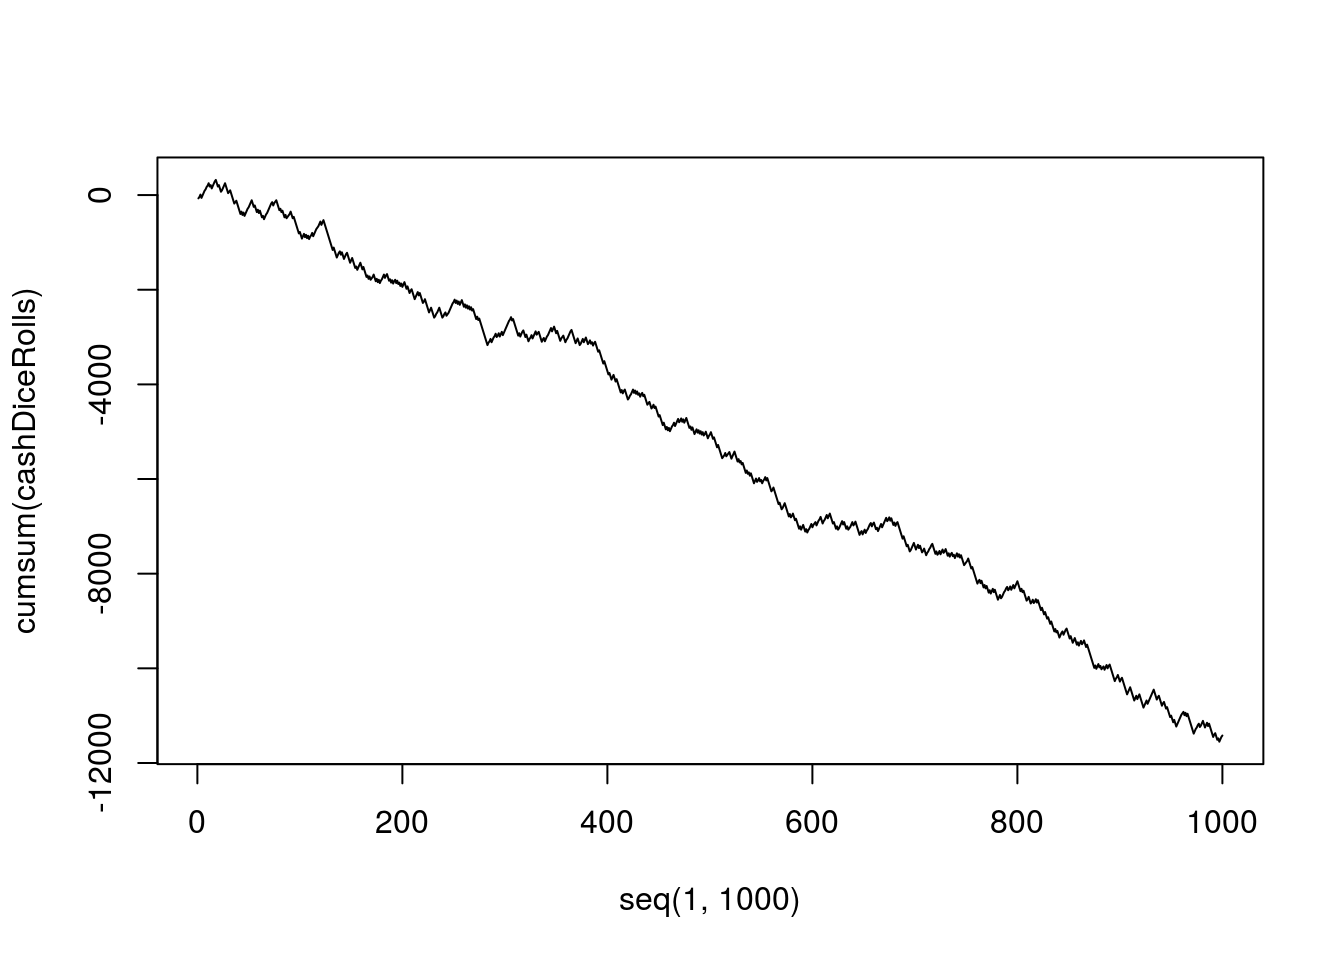
\includegraphics[width=0.6\linewidth]{BeginnersGuideToGalaxy_files/figure-latex/cassino-plot-1} 

}

\caption{How to lose cash in casino}\label{fig:cassino-plot}
\end{figure}

I think that your love to \textbf{R} is being deeper since I showed you
how it can save a lot of your money!

In nowadays stochastic analyses are more, and more popular. With
\textbf{R} it is quite easy to generate random numbers, sample and do
all the \emph{mumbo jumbo} on data. There are few functions that cover
\emph{classical} distributions: normal, Poisson, binomial, uniform (and
few others), that are actually build in base \textbf{R} distribution
(full list you will find
\href{https://stat.ethz.ch/R-manual/R-devel/library/stats/html/Distributions.html}{here}).
Some more suffisticated stuff is usually covered by some packages you
will need to download by yourself. You will easily find them by querying
Google like this
\href{https://www.google.com/search?client=ubuntu\&channel=fs\&q=Pearson+distribution+in+R\&ie=utf-8\&oe=utf-8\&gfe_rd=cr\&dcr=0\&ei=KTI5Ws_7LfPBXrSBr7gO}{Pearson
distribution in R}. By using this technique it is also possible to find
other useful libraries for dealing with distributions (try to search for
library that alows you to sample from trimmed distribution). All the
distribution libraries follow the same schema when naming functions.
They use letters: \texttt{d}, \texttt{p}, \texttt{q} and \texttt{r}
followed by abbreviation of distibution name to generate: Density,
distribution function, quantile function and random numbers --
respectively. For instance, lets generate ten random numbers from
\emph{beta distribution}, whith parameters \texttt{10} and \texttt{3}:

\begin{Shaded}
\begin{Highlighting}[]
\KeywordTok{rbeta}\NormalTok{(}\DecValTok{25}\NormalTok{,}\DecValTok{10}\NormalTok{,}\DecValTok{3}\NormalTok{)}
\end{Highlighting}
\end{Shaded}

\begin{verbatim}
##  [1] 0.8985423 0.9229588 0.9839358 0.8602257 0.8785151 0.8492233 0.7787028
##  [8] 0.7941326 0.7176832 0.8337257 0.5683864 0.5669949 0.7613561 0.6484569
## [15] 0.8416932 0.8059819 0.8935295 0.6764472 0.8259531 0.7707533 0.8651882
## [22] 0.7652365 0.7049847 0.9383397 0.8686104
\end{verbatim}

Or we can make this nice plot (Fig. \ref{fig:betaDensity-plot}) for
density of \emph{beta distribution} with parameters \texttt{8} and
\texttt{3}:

\begin{figure}

{\centering 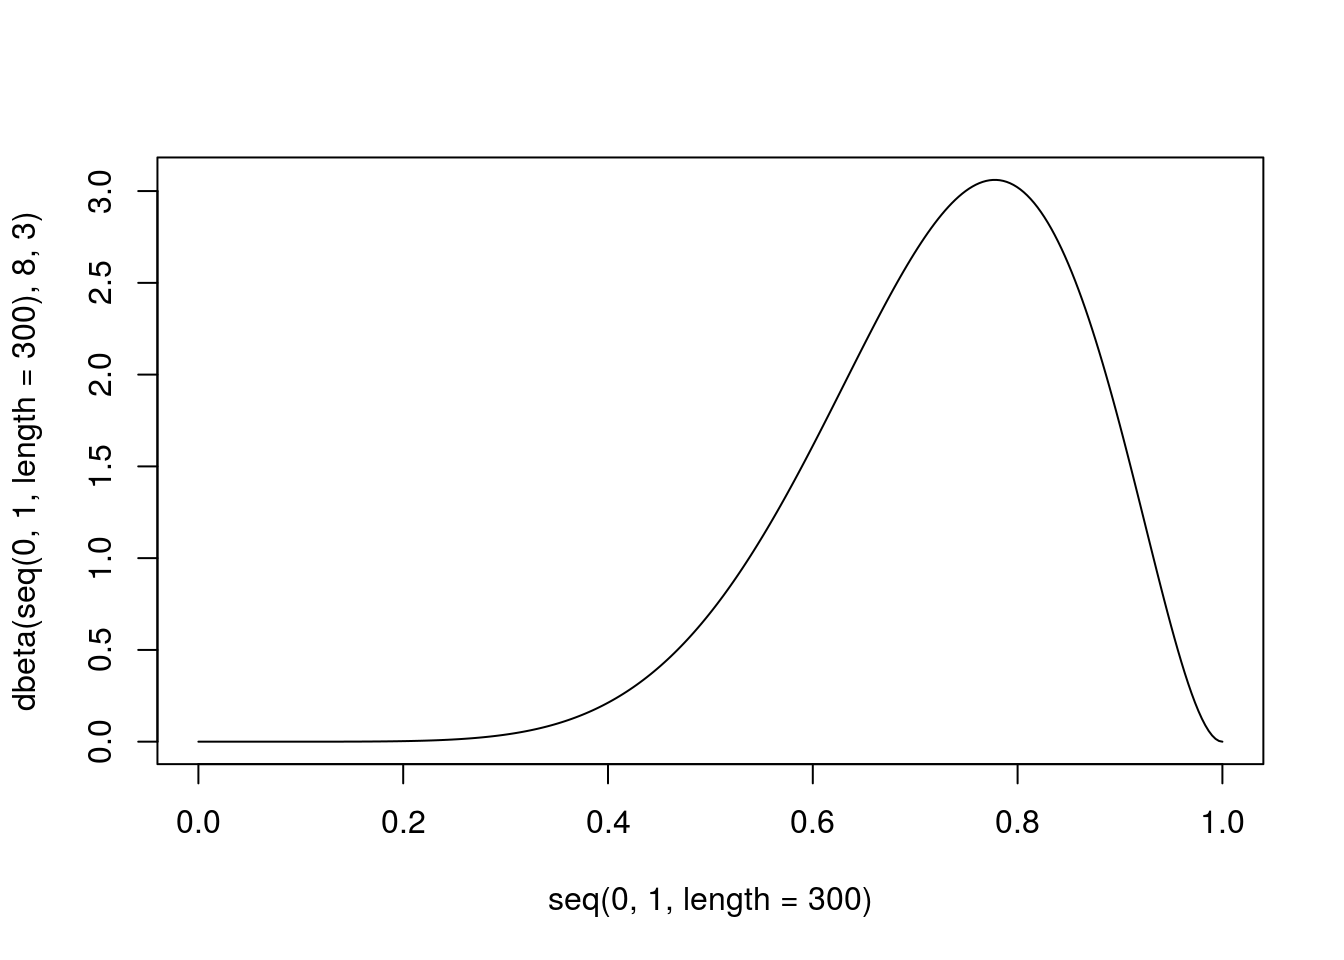
\includegraphics[width=0.6\linewidth]{BeginnersGuideToGalaxy_files/figure-latex/betaDensity-plot-1} 

}

\caption{Example of beta distribution}\label{fig:betaDensity-plot}
\end{figure}

\section{\texorpdfstring{\texttt{tidyverse} idea and \texttt{dplyr}
library}{tidyverse idea and dplyr library}}\label{tidyverse-idea-and-dplyr-library}

The whole idea of tidy data comes from one of most famous \textbf{R}
developer -- \href{http://hadley.nz/}{Hadley Wickham}. In on of his
papers \citep{hadley2014} he described procedures for generating and
cleaning data in standardized manner. Many packages right now are
designed to work best with data structured according to this
publication. Eventualy it lead to \texttt{tidiverse} -- tools tailored
for data science with common syntax and philosophy\citep{tidyverse2017}.
One of the most useful packages that are inlcuded in \texttt{tidiverse}
\citep{tidyverse2017} are \texttt{tidyr} \citep{tidyr2017} and
\texttt{dplyr} \citep{dplyr2017}. First heplps us to swap from `wide' to
`long' table format (and back). The second package contains set of tools
to easily manipulate rows, columns or even single cells in \emph{data
frame}. It is extremly powerful tool, which speeds up work with datasets
so much that after few times dealing with it, you will leave traditional
spread sheet forever.

\subsection{Wide vs.~long tables}\label{wide-vs.long-tables}

Lets start with changing wide format table into long format table.

\begin{Shaded}
\begin{Highlighting}[]
\NormalTok{wideTable <-}\StringTok{ }\KeywordTok{data.frame}\NormalTok{(}\DataTypeTok{male =} \DecValTok{1}\OperatorTok{:}\DecValTok{10}\NormalTok{, }\DataTypeTok{female =} \DecValTok{3}\OperatorTok{:}\DecValTok{12}\NormalTok{)}
\NormalTok{wideTable}
\end{Highlighting}
\end{Shaded}

\begin{verbatim}
##    male female
## 1     1      3
## 2     2      4
## 3     3      5
## 4     4      6
## 5     5      7
## 6     6      8
## 7     7      9
## 8     8     10
## 9     9     11
## 10   10     12
\end{verbatim}

Than we just make a little \emph{mumbo jumbo} and change it to long
format:

\begin{Shaded}
\begin{Highlighting}[]
\KeywordTok{library}\NormalTok{(}\StringTok{'tidyr'}\NormalTok{)}
\KeywordTok{library}\NormalTok{(}\StringTok{'magrittr'}\NormalTok{)}
\end{Highlighting}
\end{Shaded}

\begin{verbatim}
## 
## Attaching package: 'magrittr'
\end{verbatim}

\begin{verbatim}
## The following object is masked from 'package:tidyr':
## 
##     extract
\end{verbatim}

\begin{Shaded}
\begin{Highlighting}[]
\KeywordTok{library}\NormalTok{(}\StringTok{'dplyr'}\NormalTok{)}
\end{Highlighting}
\end{Shaded}

\begin{verbatim}
## 
## Attaching package: 'dplyr'
\end{verbatim}

\begin{verbatim}
## The following objects are masked from 'package:stats':
## 
##     filter, lag
\end{verbatim}

\begin{verbatim}
## The following objects are masked from 'package:base':
## 
##     intersect, setdiff, setequal, union
\end{verbatim}

\begin{Shaded}
\begin{Highlighting}[]
\NormalTok{longTable <-}\StringTok{ }\KeywordTok{gather}\NormalTok{(wideTable, }\DataTypeTok{key =}\NormalTok{ sex,}\DataTypeTok{value =}\NormalTok{ number)}
\NormalTok{longTable}
\end{Highlighting}
\end{Shaded}

\begin{verbatim}
##       sex number
## 1    male      1
## 2    male      2
## 3    male      3
## 4    male      4
## 5    male      5
## 6    male      6
## 7    male      7
## 8    male      8
## 9    male      9
## 10   male     10
## 11 female      3
## 12 female      4
## 13 female      5
## 14 female      6
## 15 female      7
## 16 female      8
## 17 female      9
## 18 female     10
## 19 female     11
## 20 female     12
\end{verbatim}

Thats how easy it But what if table is more complicated?

\begin{Shaded}
\begin{Highlighting}[]
\NormalTok{wideTable2 <-}\StringTok{ }\KeywordTok{data.frame}\NormalTok{(}\DataTypeTok{male =} \DecValTok{1}\OperatorTok{:}\DecValTok{10}\NormalTok{,}
                         \DataTypeTok{female =} \DecValTok{3}\OperatorTok{:}\DecValTok{12}\NormalTok{, }
                         \DataTypeTok{type =} \KeywordTok{rep}\NormalTok{(}\KeywordTok{c}\NormalTok{(}\StringTok{'bacteria'}\NormalTok{,}\StringTok{'virus'}\NormalTok{), }\DataTypeTok{times =} \DecValTok{5}\NormalTok{),}
                         \DataTypeTok{group =} \KeywordTok{rep}\NormalTok{(}\KeywordTok{c}\NormalTok{(}\StringTok{'a'}\NormalTok{,}\StringTok{'b'}\NormalTok{), }\DataTypeTok{each =} \DecValTok{5}\NormalTok{))}
\NormalTok{wideTable2}
\end{Highlighting}
\end{Shaded}

\begin{verbatim}
##    male female     type group
## 1     1      3 bacteria     a
## 2     2      4    virus     a
## 3     3      5 bacteria     a
## 4     4      6    virus     a
## 5     5      7 bacteria     a
## 6     6      8    virus     b
## 7     7      9 bacteria     b
## 8     8     10    virus     b
## 9     9     11 bacteria     b
## 10   10     12    virus     b
\end{verbatim}

\begin{Shaded}
\begin{Highlighting}[]
\KeywordTok{gather}\NormalTok{(wideTable2, sex, number, }\OperatorTok{-}\KeywordTok{c}\NormalTok{(}\DecValTok{3}\OperatorTok{:}\DecValTok{4}\NormalTok{))}
\end{Highlighting}
\end{Shaded}

\begin{verbatim}
##        type group    sex number
## 1  bacteria     a   male      1
## 2     virus     a   male      2
## 3  bacteria     a   male      3
## 4     virus     a   male      4
## 5  bacteria     a   male      5
## 6     virus     b   male      6
## 7  bacteria     b   male      7
## 8     virus     b   male      8
## 9  bacteria     b   male      9
## 10    virus     b   male     10
## 11 bacteria     a female      3
## 12    virus     a female      4
## 13 bacteria     a female      5
## 14    virus     a female      6
## 15 bacteria     a female      7
## 16    virus     b female      8
## 17 bacteria     b female      9
## 18    virus     b female     10
## 19 bacteria     b female     11
## 20    virus     b female     12
\end{verbatim}

In example above, using expression \texttt{-(3,4)} we indicated that we
do not want to gather columns 3 and 4.

Even more complicated?

\begin{Shaded}
\begin{Highlighting}[]
\NormalTok{wideTable3 <-}\StringTok{ }\KeywordTok{data.frame}\NormalTok{(}\DataTypeTok{male =} \KeywordTok{rep}\NormalTok{(}\DecValTok{1}\OperatorTok{:}\DecValTok{10}\NormalTok{, }\DataTypeTok{each =} \DecValTok{2}\NormalTok{),}
                         \DataTypeTok{female =} \KeywordTok{rep}\NormalTok{(}\DecValTok{3}\OperatorTok{:}\DecValTok{12}\NormalTok{, }\DataTypeTok{times =} \DecValTok{2}\NormalTok{), }
                         \DataTypeTok{type =} \KeywordTok{rep}\NormalTok{(}\KeywordTok{c}\NormalTok{(}\StringTok{'bacteria'}\NormalTok{,}\StringTok{'virus'}\NormalTok{), }\DataTypeTok{times =} \DecValTok{10}\NormalTok{),}
                         \DataTypeTok{group =} \KeywordTok{rep}\NormalTok{(}\KeywordTok{c}\NormalTok{(}\StringTok{'a'}\NormalTok{,}\StringTok{'b'}\NormalTok{), }\DataTypeTok{each =} \DecValTok{10}\NormalTok{),}
                         \DataTypeTok{day =} \DecValTok{1}\OperatorTok{:}\DecValTok{10}\NormalTok{)}
\NormalTok{wideTable3}
\end{Highlighting}
\end{Shaded}

\begin{verbatim}
##    male female     type group day
## 1     1      3 bacteria     a   1
## 2     1      4    virus     a   2
## 3     2      5 bacteria     a   3
## 4     2      6    virus     a   4
## 5     3      7 bacteria     a   5
## 6     3      8    virus     a   6
## 7     4      9 bacteria     a   7
## 8     4     10    virus     a   8
## 9     5     11 bacteria     a   9
## 10    5     12    virus     a  10
## 11    6      3 bacteria     b   1
## 12    6      4    virus     b   2
## 13    7      5 bacteria     b   3
## 14    7      6    virus     b   4
## 15    8      7 bacteria     b   5
## 16    8      8    virus     b   6
## 17    9      9 bacteria     b   7
## 18    9     10    virus     b   8
## 19   10     11 bacteria     b   9
## 20   10     12    virus     b  10
\end{verbatim}

\begin{Shaded}
\begin{Highlighting}[]
\KeywordTok{gather}\NormalTok{(wideTable3, sex, number, }\DecValTok{1}\OperatorTok{:}\DecValTok{2}\NormalTok{) }\OperatorTok\StringTok{ }\KeywordTok{spread}\NormalTok{(group, number)}
\end{Highlighting}
\end{Shaded}

\begin{verbatim}
##        type day    sex  a  b
## 1  bacteria   1 female  3  3
## 2  bacteria   1   male  1  6
## 3  bacteria   3 female  5  5
## 4  bacteria   3   male  2  7
## 5  bacteria   5 female  7  7
## 6  bacteria   5   male  3  8
## 7  bacteria   7 female  9  9
## 8  bacteria   7   male  4  9
## 9  bacteria   9 female 11 11
## 10 bacteria   9   male  5 10
## 11    virus   2 female  4  4
## 12    virus   2   male  1  6
## 13    virus   4 female  6  6
## 14    virus   4   male  2  7
## 15    virus   6 female  8  8
## 16    virus   6   male  3  8
## 17    virus   8 female 10 10
## 18    virus   8   male  4  9
## 19    virus  10 female 12 12
## 20    virus  10   male  5 10
\end{verbatim}

Here our data set had additional column \texttt{group} storing values a
and b. But imagine that \texttt{group} is not a variable, but it just
stores the names of variables - which are a and b. This somehow might be
frustrating, to decide if those are really separate variables or not.
You might run into problem, that your column named
\texttt{environmental\ factor} contains values: \emph{pH},
\emph{conductivity}, and \emph{oxygen concentration}. This would be
straightforward as each of this is different variable and you should
spread this column into three different variables. On the other hand you
might see a column that contains \emph{minimum temperature} and
\emph{maximum temperature}. This would not be as straightforward and
decision upon spreading this column would strongly depend on the
context. Nonetheless, using \texttt{spread()} function we were able to
transform values from this column as separate columns. We also used
\emph{piping operator} \texttt{\%\textgreater{}\%}. It is a shortcut
which allows us to pass the left side as an agrument to the function on
the right side of operator. In general it means that writing
\texttt{a\ \%\textgreater{}\%\ funtion(b)} actually is translated into
\texttt{function(a,b)}. In the begining this idea might be not very
usefull for you, but actually it vary helpful, mainly because your code
gets better structure and you can perform multiple operations without
storing it in variables which you do not want.

There is also one more common case that I should shortly mention -
compound variable. It is a variable that stores multiple values in a
single column. E.g. city and district, age and sex, sex and smoking,
blood type and RH, etc. With \texttt{tidyr} is very easy to deal with
it.

\begin{Shaded}
\begin{Highlighting}[]
\NormalTok{wideTable4 <-}\StringTok{ }\KeywordTok{data.frame}\NormalTok{(}\DataTypeTok{type =} \KeywordTok{rep}\NormalTok{(}\KeywordTok{c}\NormalTok{(}\StringTok{'bacteria.a'}\NormalTok{,}\StringTok{'virus.a'}\NormalTok{), }\DataTypeTok{times =} \DecValTok{5}\NormalTok{))}
\NormalTok{wideTable4}
\end{Highlighting}
\end{Shaded}

\begin{verbatim}
##          type
## 1  bacteria.a
## 2     virus.a
## 3  bacteria.a
## 4     virus.a
## 5  bacteria.a
## 6     virus.a
## 7  bacteria.a
## 8     virus.a
## 9  bacteria.a
## 10    virus.a
\end{verbatim}

\begin{Shaded}
\begin{Highlighting}[]
\NormalTok{wideTable4 }\OperatorTok\StringTok{ }\KeywordTok{separate}\NormalTok{(type, }\KeywordTok{c}\NormalTok{(}\StringTok{'organism'}\NormalTok{, }\StringTok{'type'}\NormalTok{), }\DataTypeTok{sep =} \StringTok{'}\CharTok{\textbackslash{}\textbackslash{}}\StringTok{.'}\NormalTok{)}
\end{Highlighting}
\end{Shaded}

\begin{verbatim}
##    organism type
## 1  bacteria    a
## 2     virus    a
## 3  bacteria    a
## 4     virus    a
## 5  bacteria    a
## 6     virus    a
## 7  bacteria    a
## 8     virus    a
## 9  bacteria    a
## 10    virus    a
\end{verbatim}

\subsection{\texorpdfstring{World of
\texttt{dplyr}}{World of dplyr}}\label{world-of-dplyr}

\texttt{dplyr} is a library containing several useful functions,
designed to ease all kinds of transformations, selections and filtering
of your data frame. As the number and possibilities of functions are
really huge, here I will concentrate only on some mostly used ones. Of
course there is a well described documentation if you want to get
deeper.

\subsubsection{\texorpdfstring{\texttt{select} columns and
\texttt{filter}
rows}{select columns and filter rows}}\label{select-columns-and-filter-rows}

Those are the most basic operations on data frames. \texttt{select()}
function allows you to choose which columns you use. The biggest
advantege of using this function instead of simple addressing, is that
you can use some special functions inside it:
\texttt{starts\_with(),\ ends\_with(),\ contains(),\ matches(),\ num\_range()}
which are helpful when using big data sets with numerous columns. There
is also similar function \texttt{rename()} which can be used to change
variable names, but in results (contrary to \texttt{select()}) it keeps
all the variables. Lets look how the thing works on some simple
examples:

\begin{Shaded}
\begin{Highlighting}[]
\KeywordTok{head}\NormalTok{(}\KeywordTok{select}\NormalTok{(wideTable3, }\KeywordTok{starts_with}\NormalTok{(}\StringTok{'gr'}\NormalTok{)), }\DecValTok{3}\NormalTok{)}
\end{Highlighting}
\end{Shaded}

\begin{verbatim}
##   group
## 1     a
## 2     a
## 3     a
\end{verbatim}

\begin{Shaded}
\begin{Highlighting}[]
\KeywordTok{head}\NormalTok{(}\KeywordTok{select}\NormalTok{(wideTable3, }\OperatorTok{-}\KeywordTok{starts_with}\NormalTok{(}\StringTok{'gr'}\NormalTok{)), }\DecValTok{3}\NormalTok{)}
\end{Highlighting}
\end{Shaded}

\begin{verbatim}
##   male female     type day
## 1    1      3 bacteria   1
## 2    1      4    virus   2
## 3    2      5 bacteria   3
\end{verbatim}

\begin{Shaded}
\begin{Highlighting}[]
\KeywordTok{head}\NormalTok{(}\KeywordTok{select}\NormalTok{(wideTable3, }\KeywordTok{contains}\NormalTok{(}\StringTok{'ale'}\NormalTok{)), }\DecValTok{3}\NormalTok{)}
\end{Highlighting}
\end{Shaded}

\begin{verbatim}
##   male female
## 1    1      3
## 2    1      4
## 3    2      5
\end{verbatim}

\begin{Shaded}
\begin{Highlighting}[]
\KeywordTok{head}\NormalTok{(}\KeywordTok{rename}\NormalTok{(wideTable3, }\DataTypeTok{Male =}\NormalTok{ male), }\DecValTok{3}\NormalTok{)}
\end{Highlighting}
\end{Shaded}

\begin{verbatim}
##   Male female     type group day
## 1    1      3 bacteria     a   1
## 2    1      4    virus     a   2
## 3    2      5 bacteria     a   3
\end{verbatim}

Filtering rows is also straightforward. Inside function
\texttt{filter()} you cand use logical operators
(\texttt{\&,\ \textbar{},\ xor,\ !}), comparisions (e.g. \texttt{==} or
\texttt{\textgreater{}=}), or functions
(\texttt{is.na(),\ between(),\ near()}).

\begin{Shaded}
\begin{Highlighting}[]
\KeywordTok{filter}\NormalTok{(wideTable3, group }\OperatorTok{==}\StringTok{ 'a'}\NormalTok{)}
\end{Highlighting}
\end{Shaded}

\begin{verbatim}
##    male female     type group day
## 1     1      3 bacteria     a   1
## 2     1      4    virus     a   2
## 3     2      5 bacteria     a   3
## 4     2      6    virus     a   4
## 5     3      7 bacteria     a   5
## 6     3      8    virus     a   6
## 7     4      9 bacteria     a   7
## 8     4     10    virus     a   8
## 9     5     11 bacteria     a   9
## 10    5     12    virus     a  10
\end{verbatim}

\begin{Shaded}
\begin{Highlighting}[]
\KeywordTok{filter}\NormalTok{(wideTable3, type }\OperatorTok{!=}\StringTok{ 'bacteria'}\NormalTok{)}
\end{Highlighting}
\end{Shaded}

\begin{verbatim}
##    male female  type group day
## 1     1      4 virus     a   2
## 2     2      6 virus     a   4
## 3     3      8 virus     a   6
## 4     4     10 virus     a   8
## 5     5     12 virus     a  10
## 6     6      4 virus     b   2
## 7     7      6 virus     b   4
## 8     8      8 virus     b   6
## 9     9     10 virus     b   8
## 10   10     12 virus     b  10
\end{verbatim}

\begin{Shaded}
\begin{Highlighting}[]
\KeywordTok{filter}\NormalTok{(wideTable3, }\KeywordTok{near}\NormalTok{(female, }\DecValTok{5}\NormalTok{))}
\end{Highlighting}
\end{Shaded}

\begin{verbatim}
##   male female     type group day
## 1    2      5 bacteria     a   3
## 2    7      5 bacteria     b   3
\end{verbatim}

\subsection{\texorpdfstring{\texttt{mutate} and
\texttt{transmute}}{mutate and transmute}}\label{mutate-and-transmute}

Both functions are widly used in data manipulation in \textbf{R}. Their
main purpose is to create new variable (usually from existing ones) in
data frame. Lets look on examples:

\begin{Shaded}
\begin{Highlighting}[]
\KeywordTok{select}\NormalTok{(wideTable3, male) }\OperatorTok
\StringTok{  }\KeywordTok{mutate}\NormalTok{(}\DataTypeTok{cumulativeMaleSum =} \KeywordTok{cumsum}\NormalTok{(male)) }\OperatorTok
\StringTok{  }\KeywordTok{head}\NormalTok{(}\DecValTok{5}\NormalTok{)}
\end{Highlighting}
\end{Shaded}

\begin{verbatim}
##   male cumulativeMaleSum
## 1    1                 1
## 2    1                 2
## 3    2                 4
## 4    2                 6
## 5    3                 9
\end{verbatim}

\begin{Shaded}
\begin{Highlighting}[]
\KeywordTok{select}\NormalTok{(wideTable3, male, female) }\OperatorTok
\StringTok{  }\KeywordTok{mutate}\NormalTok{(}\DataTypeTok{cumulativeMaleSum =} \KeywordTok{cumsum}\NormalTok{(male),}
         \DataTypeTok{femaleLog =} \KeywordTok{log}\NormalTok{(female),}
         \DataTypeTok{cumSumFemaleLog =} \KeywordTok{cumsum}\NormalTok{(femaleLog)) }\OperatorTok
\StringTok{  }\KeywordTok{head}\NormalTok{(}\DecValTok{5}\NormalTok{)}
\end{Highlighting}
\end{Shaded}

\begin{verbatim}
##   male female cumulativeMaleSum femaleLog cumSumFemaleLog
## 1    1      3                 1  1.098612        1.098612
## 2    1      4                 2  1.386294        2.484907
## 3    2      5                 4  1.609438        4.094345
## 4    2      6                 6  1.791759        5.886104
## 5    3      7                 9  1.945910        7.832014
\end{verbatim}

As you can see in second example, when we use \texttt{mutate()}
function, the newly created variables (in this example
\texttt{femaleLog}) are available immediately so we can use them to
create another variable (in this case \texttt{cumSumFemaleLog}) within
one function call. In this example, I also used piping operator, becasue
calculating intermediate steps and storing them as a result, which can
be used later is useless as we are interested only in final outcome. The
biggest advantage of this procedure is that we clean our
\emph{Environment} clean and preserve memomry -- which is very important
in long and memory consuming projects. Last but not least, the
difference between \texttt{mutate()} and \texttt{transmute()} is that
the latter do not preserve all variables, only the ones you created.

\subsubsection{\texorpdfstring{\texttt{group\_by} and
\texttt{summarise}}{group\_by and summarise}}\label{group_by-and-summarise}

\texttt{summarise()} is commonly used function on grouped data. It
allows to calculate many typical descriptive statistics (like
\texttt{mean()} or \texttt{quantile}) for particular groups in you data
set, as well as it can count number of observations (\texttt{n()}
function), or number of uniqe observations (\texttt{distinct()}). To see
how it works in practice lets look back on our example and calculate
mean value for \texttt{males} and \texttt{female}, as well as day range
and number of cases for groups derived from \texttt{type}.

\begin{Shaded}
\begin{Highlighting}[]
\NormalTok{wideTable3 }\OperatorTok\StringTok{ }
\StringTok{  }\KeywordTok{group_by}\NormalTok{(type) }\OperatorTok\StringTok{ }
\StringTok{  }\KeywordTok{summarise}\NormalTok{(}\DataTypeTok{meanF =} \KeywordTok{mean}\NormalTok{(female),}
            \DataTypeTok{meanM =} \KeywordTok{mean}\NormalTok{(male),}
            \DataTypeTok{numberOfDays =}\NormalTok{ (}\KeywordTok{range}\NormalTok{(day)[}\DecValTok{2}\NormalTok{]}\OperatorTok{-}\KeywordTok{range}\NormalTok{(day)[}\DecValTok{1}\NormalTok{]),}
            \DataTypeTok{numberOfCases =} \KeywordTok{n}\NormalTok{())}
\end{Highlighting}
\end{Shaded}

\begin{verbatim}
## # A tibble: 2 x 5
##   type     meanF meanM numberOfDays numberOfCases
##   <fctr>   <dbl> <dbl>        <int>         <int>
## 1 bacteria  7.00  5.50            8            10
## 2 virus     8.00  5.50            8            10
\end{verbatim}

Easy.

\subsubsection{\texorpdfstring{Is there anything more in \texttt{dplyr}
library?}{Is there anything more in dplyr library?}}\label{is-there-anything-more-in-dplyr-library}

Yes. Actually I presented here only very very tiny fracture of
\texttt{dplyr} possibilities just to familiarize you with syntax and
using piping operator. When you go deeper into world of data frames
transformation, you will find other commonly used functions like:
different kinds of joining data frames (simmilar to SQL joining tables),
conditional selecting, filtering, renaming rows and columns, extracting
values or arranging your data frame. Thankfuly this procedures are so
common that even if you won't grasp it immedately from functions
description, you will still find hundreds of tutorials on the web, or
help in \emph{StackOverflow}.

\chapter{Lets do some math!}\label{lets-do-some-math}

\section{Simple statistical model}\label{simple-statistical-model}

Ok. There is no such thing as simple statistical model. However there
are lots of packages that will make you suffer less. In fact this is one
of biggest \textbf{R} advantages, that you can make even very
suffisticated statistical modelling without any knowledge on programming
since you use \emph{black boxes}. When you are dealing with classic
statistical models many of them are included in \textbf{base R}
distribution - like linear or gereralized additive models. You would
probably need to use mixed effect models, at some point. Good news is
that there is a very nice and quite straightforward to use library
called \texttt{lme4} . Every time you run into problem, and you do not
know what to use for statistical modelling, or how to perform full
procedure, just query google. There are hundrets of blogs, web pages and
\emph{Stack Overflow} discussion on it.

\section{Other models}\label{other-models}

\subsection{Libraries}\label{libraries}

Other, usually dynamic models require more knowledge, experience and
some libraries. Before you start looking for more tailored solutions,
install following libraries: \texttt{deSolve}, \texttt{fitdistrplus},
\texttt{rriskDistributions} and \texttt{truncdist}. First one contains
tools for solving differential equations sets, second and third provides
you tools to deal with distriubutions (such as comparing distributions
or estimating its parameters), and the last one allows you to use
truncated distributions.

\subsection{Simple asymptotic model and
noise}\label{simple-asymptotic-model-and-noise}

\subsection{\texorpdfstring{Mechanistic model in
\textbf{R}}{Mechanistic model in R}}\label{mechanistic-model-in-r}

\subsection{Solving differential
equations}\label{solving-differential-equations}

\chapter{Functions}\label{functions-1}

In short, function is a piece of code that takes some arguments, makes
\emph{mumbo jumbo} and returns result. All the time, through this book
we were using functions that are buil in \textbf{base R} or comes from
additional packages (like \texttt{dplyr}). So you are now quite familiar
whit the syntax that resambles typical mathematical syntax -- \emph{name
of a function followed by arguments in brackets - like f(x)}. From time
to time you will need to do something in your code for few times with
different arguments. In order to not repeat yourself and not \emph{copy
-- paste} your code multiple times you can wrap your procedure in a
function. The best way (as always) to understand how to do it, is to do
it. To begin with something simple we will start with makeing basic math
functions which later will lead us to simple calculator.

\section{Simple math functions.}\label{simple-math-functions.}

Simple math operations include: \emph{adding}, \emph{substracting},
\emph{dividing} and \emph{multipling}. To make our calculator slightly
less boring, we can also add \emph{powers} and \emph{nth rooting}. To
not to complicate to much things in the begining, lets say that we want
our function to take two and only two arguments. Lets look below how to
code our functions:

\begin{Shaded}
\begin{Highlighting}[]
\NormalTok{addF <-}\StringTok{ }\ControlFlowTok{function}\NormalTok{(x,y) \{}
  \KeywordTok{return}\NormalTok{(x}\OperatorTok{+}\NormalTok{y)}
\NormalTok{\}}
\NormalTok{subF <-}\StringTok{ }\ControlFlowTok{function}\NormalTok{(x,y) \{}
  \KeywordTok{return}\NormalTok{(x}\OperatorTok{-}\NormalTok{y)}
\NormalTok{\}}
\NormalTok{divF <-}\StringTok{ }\ControlFlowTok{function}\NormalTok{(x,y) \{}
  \KeywordTok{return}\NormalTok{(x}\OperatorTok{/}\NormalTok{y)}
\NormalTok{\}}
\NormalTok{mulF <-}\StringTok{ }\ControlFlowTok{function}\NormalTok{(x,y) \{}
  \KeywordTok{return}\NormalTok{(x}\OperatorTok{*}\NormalTok{y)}
\NormalTok{\}}
\NormalTok{powF <-}\StringTok{ }\ControlFlowTok{function}\NormalTok{(x,y) \{}
  \KeywordTok{return}\NormalTok{(x}\OperatorTok{:}\NormalTok{y)}
\NormalTok{\}}
\NormalTok{ntrF <-}\StringTok{ }\ControlFlowTok{function}\NormalTok{(x,y) \{}
  \KeywordTok{return}\NormalTok{(x}\OperatorTok{^}\NormalTok{(}\DecValTok{1}\OperatorTok{/}\NormalTok{y))}
\NormalTok{\}}
\end{Highlighting}
\end{Shaded}

\section{Building your own
calculator}\label{building-your-own-calculator}

Above example is of course useless and boring. So lets quickly get to
making calculator, that would use one of above functions, or return
results of all of them. So actually this time we will make so called
\emph{wraper} around previously made functions. We will use
\emph{switch} functionality, so besides our two parameters: \texttt{x}
and \texttt{y} we will also tell our function which of the results we
are interested in.

\begin{Shaded}
\begin{Highlighting}[]
\NormalTok{simpleCalculator <-}\StringTok{ }\ControlFlowTok{function}\NormalTok{(x, y, mathType) \{}
\NormalTok{  addF <-}\StringTok{ }\ControlFlowTok{function}\NormalTok{(x, y) \{}
  \KeywordTok{return}\NormalTok{(x}\OperatorTok{+}\NormalTok{y)}
\NormalTok{  \}}
\NormalTok{  subF <-}\StringTok{ }\ControlFlowTok{function}\NormalTok{(x, y) \{}
  \KeywordTok{return}\NormalTok{(x}\OperatorTok{-}\NormalTok{y)}
\NormalTok{  \}}
\NormalTok{  divF <-}\StringTok{ }\ControlFlowTok{function}\NormalTok{(x, y) \{}
  \KeywordTok{return}\NormalTok{(x}\OperatorTok{/}\NormalTok{y)}
\NormalTok{  \}}
\NormalTok{  mulF <-}\StringTok{ }\ControlFlowTok{function}\NormalTok{(x, y) \{}
  \KeywordTok{return}\NormalTok{(x}\OperatorTok{*}\NormalTok{y)}
\NormalTok{  \}}
\NormalTok{  powF <-}\StringTok{ }\ControlFlowTok{function}\NormalTok{(x, y) \{}
  \KeywordTok{return}\NormalTok{(x}\OperatorTok{^}\NormalTok{y)}
\NormalTok{  \}}
\NormalTok{  ntrF <-}\StringTok{ }\ControlFlowTok{function}\NormalTok{(x, y) \{}
  \KeywordTok{return}\NormalTok{(x}\OperatorTok{^}\NormalTok{(}\DecValTok{1}\OperatorTok{/}\NormalTok{y))}
\NormalTok{  \}}
  \ControlFlowTok{switch}\NormalTok{(mathType,}
         \DataTypeTok{add =} \KeywordTok{addF}\NormalTok{(x, y),}
         \DataTypeTok{substract =} \KeywordTok{subF}\NormalTok{(x, y),}
         \DataTypeTok{multiple =} \KeywordTok{mulF}\NormalTok{(x, y),}
         \DataTypeTok{divide =} \KeywordTok{divF}\NormalTok{(x, y),}
         \DataTypeTok{power =} \KeywordTok{powF}\NormalTok{(x, y),}
         \DataTypeTok{root =} \KeywordTok{ntrF}\NormalTok{(x, y),}
         \DataTypeTok{all =} \KeywordTok{cat}\NormalTok{(}\StringTok{'The result of mathematical opereators on two numbers:'}\NormalTok{,}
                      \KeywordTok{paste}\NormalTok{(x, }\StringTok{'and'}\NormalTok{, y), }\StringTok{'are:'}\NormalTok{, }\StringTok{'}\CharTok{\textbackslash{}n}\StringTok{addition:'}\NormalTok{, }\KeywordTok{addF}\NormalTok{(x, y),}
                      \StringTok{'}\CharTok{\textbackslash{}n}\StringTok{substraction:'}\NormalTok{, }\KeywordTok{subF}\NormalTok{(x, y), }\StringTok{'}\CharTok{\textbackslash{}n}\StringTok{multiplication:'}\NormalTok{, }\KeywordTok{mulF}\NormalTok{(x, y),}
                      \StringTok{'}\CharTok{\textbackslash{}n}\StringTok{dvision:'}\NormalTok{, }\KeywordTok{divF}\NormalTok{(x, y), }\StringTok{'}\CharTok{\textbackslash{}n}\StringTok{What is more the'}\NormalTok{, y,}
                      \StringTok{'th power of'}\NormalTok{, x, }\StringTok{'is'}\NormalTok{, }\KeywordTok{powF}\NormalTok{(x, y), }\StringTok{'and'}\NormalTok{, x, y,}
                      \StringTok{'th root is'}\NormalTok{, }\KeywordTok{ntrF}\NormalTok{(x, y)))}
\NormalTok{\}}

\KeywordTok{simpleCalculator}\NormalTok{(}\DecValTok{25}\NormalTok{,}\DecValTok{5}\NormalTok{, }\StringTok{'root'}\NormalTok{)}
\end{Highlighting}
\end{Shaded}

\begin{verbatim}
## [1] 1.903654
\end{verbatim}

\begin{Shaded}
\begin{Highlighting}[]
\KeywordTok{simpleCalculator}\NormalTok{(}\DecValTok{16}\NormalTok{,}\DecValTok{2}\NormalTok{,}\StringTok{'all'}\NormalTok{)}
\end{Highlighting}
\end{Shaded}

\begin{verbatim}
## The result of mathematical opereators on two numbers: 16 and 2 are: 
## addition: 18 
## substraction: 14 
## multiplication: 32 
## dvision: 8 
## What is more the 2 th power of 16 is 256 and 16 2 th root is 4
\end{verbatim}

\section{\texorpdfstring{It is not over yet\ldots{} \emph{Calculator
shouldn't divide be
0}!}{It is not over yet\ldots{} Calculator shouldn't divide be 0!}}\label{it-is-not-over-yet-calculator-shouldnt-divide-be-0}

We know that division by 0 is not the best idea in the world, thus we
should stop users (or ourselves) from doing it. Thus we will add an
\texttt{if...else} statment to our function. Next time when you use 0 as
a second argument you will see an error. Also, we declare
\texttt{mathType\ =\ \textquotesingle{}all\textquotesingle{}} as a
default value, so if we omit this parameter, function will evaluate
anyway.

\begin{Shaded}
\begin{Highlighting}[]
\NormalTok{simpleCalculator <-}\StringTok{ }\ControlFlowTok{function}\NormalTok{(x, y, }\DataTypeTok{mathType =} \StringTok{'all'}\NormalTok{) \{}
  \ControlFlowTok{if}\NormalTok{ (mathType }\OperatorTok{==}\StringTok{ 'divide'} \OperatorTok{&}\StringTok{ }\NormalTok{y }\OperatorTok{==}\StringTok{ }\DecValTok{0}\NormalTok{) \{}
    \KeywordTok{return}\NormalTok{(}\StringTok{'You cannot divide by 0, please change y value.'}\NormalTok{)}
\NormalTok{  \} }\ControlFlowTok{else} \ControlFlowTok{if}\NormalTok{ (mathType }\OperatorTok{==}\StringTok{ 'root'} \OperatorTok{&}\StringTok{ }\NormalTok{y }\OperatorTok{==}\StringTok{ }\DecValTok{0}\NormalTok{) \{}
    \KeywordTok{return}\NormalTok{(}\StringTok{'Root denominator is 0, cannot perform operation, please change y value.'}\NormalTok{)}
\NormalTok{  \} }\ControlFlowTok{else} \ControlFlowTok{if}\NormalTok{ (mathType }\OperatorTok{==}\StringTok{ 'all'} \OperatorTok{&}\StringTok{ }\NormalTok{y }\OperatorTok{==}\StringTok{ }\DecValTok{0}\NormalTok{) \{}
    \KeywordTok{return}\NormalTok{(}\StringTok{'Y value needs to be different from 0 to make division and nth root.'}\NormalTok{)}
\NormalTok{  \}}
\NormalTok{  addF <-}\StringTok{ }\ControlFlowTok{function}\NormalTok{(x, y) \{}
  \KeywordTok{return}\NormalTok{(x}\OperatorTok{+}\NormalTok{y)}
\NormalTok{  \}}
\NormalTok{  subF <-}\StringTok{ }\ControlFlowTok{function}\NormalTok{(x, y) \{}
  \KeywordTok{return}\NormalTok{(x}\OperatorTok{-}\NormalTok{y)}
\NormalTok{  \}}
\NormalTok{  divF <-}\StringTok{ }\ControlFlowTok{function}\NormalTok{(x, y) \{}
  \KeywordTok{return}\NormalTok{(x}\OperatorTok{/}\NormalTok{y)}
\NormalTok{  \}}
\NormalTok{  mulF <-}\StringTok{ }\ControlFlowTok{function}\NormalTok{(x, y) \{}
  \KeywordTok{return}\NormalTok{(x}\OperatorTok{*}\NormalTok{y)}
\NormalTok{  \}}
\NormalTok{  powF <-}\StringTok{ }\ControlFlowTok{function}\NormalTok{(x, y) \{}
  \KeywordTok{return}\NormalTok{(x}\OperatorTok{^}\NormalTok{y)}
\NormalTok{  \}}
\NormalTok{  ntrF <-}\StringTok{ }\ControlFlowTok{function}\NormalTok{(x, y) \{}
  \KeywordTok{return}\NormalTok{(x}\OperatorTok{^}\NormalTok{(}\DecValTok{1}\OperatorTok{/}\NormalTok{y))}
\NormalTok{  \}}
  \ControlFlowTok{switch}\NormalTok{(mathType,}
         \DataTypeTok{add =} \KeywordTok{addF}\NormalTok{(x, y),}
         \DataTypeTok{substract =} \KeywordTok{subF}\NormalTok{(x, y),}
         \DataTypeTok{multiple =} \KeywordTok{mulF}\NormalTok{(x, y),}
         \DataTypeTok{divide =} \KeywordTok{divF}\NormalTok{(x, y),}
         \DataTypeTok{power =} \KeywordTok{powF}\NormalTok{(x, y),}
         \DataTypeTok{root =} \KeywordTok{ntrF}\NormalTok{(x, y),}
         \DataTypeTok{all =} \KeywordTok{cat}\NormalTok{(}\StringTok{'The result of mathematical opereators on two numbers:'}\NormalTok{,}
                      \KeywordTok{paste}\NormalTok{(x, }\StringTok{'and'}\NormalTok{, y), }\StringTok{'are:'}\NormalTok{, }\StringTok{'}\CharTok{\textbackslash{}n}\StringTok{addition:'}\NormalTok{, }\KeywordTok{addF}\NormalTok{(x, y),}
                      \StringTok{'}\CharTok{\textbackslash{}n}\StringTok{substraction:'}\NormalTok{, }\KeywordTok{subF}\NormalTok{(x, y), }\StringTok{'}\CharTok{\textbackslash{}n}\StringTok{multiplication:'}\NormalTok{, }\KeywordTok{mulF}\NormalTok{(x, y),}
                      \StringTok{'}\CharTok{\textbackslash{}n}\StringTok{dvision:'}\NormalTok{, }\KeywordTok{divF}\NormalTok{(x, y), }\StringTok{'}\CharTok{\textbackslash{}n}\StringTok{What is more the'}\NormalTok{, y,}
                      \StringTok{'th power of'}\NormalTok{, x, }\StringTok{'is'}\NormalTok{, }\KeywordTok{powF}\NormalTok{(x, y), }\StringTok{'and'}\NormalTok{, x, y,}
                      \StringTok{'th root is'}\NormalTok{, }\KeywordTok{ntrF}\NormalTok{(x, y)))}

\NormalTok{\}}
\KeywordTok{simpleCalculator}\NormalTok{(}\DecValTok{25}\NormalTok{,}\DecValTok{0}\NormalTok{)}
\end{Highlighting}
\end{Shaded}

\begin{verbatim}
## [1] "Y value needs to be different from 0 to make division and nth root."
\end{verbatim}

\begin{Shaded}
\begin{Highlighting}[]
\KeywordTok{simpleCalculator}\NormalTok{(}\DecValTok{25}\NormalTok{,}\DecValTok{0}\NormalTok{, }\StringTok{'root'}\NormalTok{)}
\end{Highlighting}
\end{Shaded}

\begin{verbatim}
## [1] "Root denominator is 0, cannot perform operation, please change y value."
\end{verbatim}

\begin{Shaded}
\begin{Highlighting}[]
\KeywordTok{simpleCalculator}\NormalTok{(}\DecValTok{25}\NormalTok{,}\DecValTok{0}\NormalTok{, }\StringTok{'divide'}\NormalTok{)}
\end{Highlighting}
\end{Shaded}

\begin{verbatim}
## [1] "You cannot divide by 0, please change y value."
\end{verbatim}

\begin{Shaded}
\begin{Highlighting}[]
\KeywordTok{simpleCalculator}\NormalTok{(}\DecValTok{25}\NormalTok{,}\DecValTok{5}\NormalTok{)}
\end{Highlighting}
\end{Shaded}

\begin{verbatim}
## The result of mathematical opereators on two numbers: 25 and 5 are: 
## addition: 30 
## substraction: 20 
## multiplication: 125 
## dvision: 5 
## What is more the 5 th power of 25 is 9765625 and 25 5 th root is 1.903654
\end{verbatim}

\chapter{Graphics}\label{graphics}

What would be our work value without visualisation? Not much. \textbf{R}
provides use with some tools to make plots, charst and other visual
stuff. However base version has very limited graphic design by default
and making it pretty needs a lot of time and code. Nowadays, however, in
\texttt{tidyverse} there is a very powerfull library with dozens of
extensions - \texttt{ggplot2}. \emph{GG} stands for \emph{Gramar of
Graphics} and in parctice it means that we build our visualisation layer
after layer.

\chapter{Final indications}\label{final-indications}

\section{Use Projects}\label{use-projects}

To organize your work, not only in \textbf{RStudio}, but also on hard
drive you should use projects. It is extremly easy in this IDE. Just
click button -- \emph{Create new project} -- choose \emph{New Directory}
and type of project you need. \textbf{RStudio} will take care of
everything for you. Later you can easily add files of subfolders with
specifing content into your project and use ralational links.

\section{Use RMarkodow}\label{use-rmarkodow}

To make your work more reproductible, and also to make nice looking
output (in html or pdf) it is a good idea to work in RMarkdown files
instead of RScripts. The syntax of \textbf{RMarkdown} is nearly
identical to original \textbf{Markdown}, but allows you to execute and
store \textbf{RCode}. You can find
\href{http://rmarkdown.rstudio.com/articles_intro.html}{RMarkdown
introduction here}. There is also nice
\href{https://www.rstudio.com/wp-content/uploads/2015/02/rmarkdown-cheatsheet.pdf}{cheat
sheet} which contains all commands you will need. As there is strong
pressure to make reasearch and science more open and reproductible, it
is strongly adviced that you work with proper tools to do it like
\textbf{RMarkdown} or \textbf{Project Jupyter}. If you want to learn
more, there is very nice
\href{https://www.britishecologicalsociety.org/wp-content/uploads/2017/12/guide-to-reproducible-code.pdf}{guide
by British Ecological Society} you should read.

\section{Use .rds files}\label{use-.rds-files}

Usually we work with plain text files like csv or tsv in \textbf{R}.
Howevere, there is also a highly valuable format of files caled rds,
that makes work even more pleasant. It not only preserves all classes of
variables, but also takes less space than plain text file, due to
compression algorithms. Also when using \texttt{saveRDS()} you don't
need to define hundrets of parameters, just name of object you want to
save and its file name. The downside is that it is format to use
directly with R.

\bibliography{book.bib,packages.bib}


\end{document}
